\documentclass[12pt]{article}
\usepackage{amsmath}
\usepackage{amssymb}
\usepackage{graphicx}
\usepackage{subcaption}
\usepackage{cite}
\usepackage{float}
\usepackage{listings}
\usepackage{minted}
\usepackage{comment}
\usepackage{xcolor}
\usepackage{hyperref} % Load hyperref last


\hypersetup{
    colorlinks=true,
    linkcolor=black,   % Color of internal links (e.g., toc, sections, etc.)
    citecolor=black,   % Color of citation links (e.g., bibliography)
    urlcolor=black     % Color of external links (e.g., URLs)
}

\title{Path Tracing Renderer Using Monte Carlo Methods}
\author{Silas Maughan}
\date{\today}

\begin{document}

\maketitle
\begin{abstract}
    This report presents an expository on the foundational mathematical knowledge and implementation of a path tracing renderer using Monte Carlo methods to simulate realistic lighting in a 3D scene. Various sampling and variance reduction methods are explored to enhance image quality and convergence speed. Experimental results demonstrate the effectiveness of these techniques in reducing noise and improving rendering efficiency.
\end{abstract}

\tableofcontents
\break
\section{Introduction}
\label{sec:intro}
\subsection{Purpose and Scope}
\subsubsection{Goals of the Document}

This expository aims to achieve the following objectives:
\begin{enumerate}
    \item To comprehensively analyse of the \textit{mathematical} foundations underlying path tracing, creating a scene, and Monte Carlo integration techniques.

    \item To demonstrate the \textit{visual} impact of Monte Carlo methods in path tracing for realistic light simulation, exploring their impact on image fidelity, convergence rates, and rendering efficiency.

    \item To elucidate the \textit{design} and implementation of a path tracing system, with particular emphasis on adhering to software modelling principles and real-time visualisation with OpenGL.
\end{enumerate}

Through these objectives, this document seeks to offer a thorough exploration of path tracing, from its mathematical underpinnings to its practical realization in computer graphics, serving as a valuable resource for researchers and practitioners in the field of physically-based rendering.

\subsubsection{Overview of the Methodological Approach}
This expository adopts a progressive approach to path-tracing principles and implementation.
We begin by examining the foundational elements of a generic path tracer, including ray representation, intersection testing, and basic shading models. We present the underlying mathematical principles for each of these components, followed by their corresponding representations. This foundational phase establishes the core concepts upon which more advanced techniques are built.

Building upon these foundational elements, we abstract the lighting simulation process into a comprehensive mathematical framework. This transition allows us to view the path-tracing problem as an integration task. We introduce Monte Carlo methods as a powerful tool for numerical integration, exploring how these statistical techniques can be applied to solve the rendering equation efficiently.

As we introduce each component, we demonstrate its effect on the rendered image, allowing for a clear understanding of how theoretical concepts translate to visual outcomes. This iterative approach provides immediate feedback on the impact of each implemented feature, reinforcing the connection between mathematical principles and their applications in computer graphics.

\subsection{Background}
\subsubsection{Overview of Ray Tracing}
Ray tracing is a rendering technique that simulates the physical behaviour of light to create realistic images. At its core, ray tracing involves tracing the path of light rays as they interact with objects in a virtual scene \cite{Glassner1989}.
The fundamental concept is to cast rays from a virtual camera through each pixel of an image plane into the scene. These rays interact with objects, potentially reflecting, refracting, or being absorbed, mimicking the behaviour of light in the real world. By accurately modelling these interactions, ray tracing can produce highly realistic effects such as shadows, reflections, and refractions.

Path tracing, an advanced form of ray tracing, extends this concept by using Monte Carlo methods to solve the rendering equation \cite{Kajiya1986}. It traces numerous light paths through the scene, accounting for multiple bounces and complex light interactions. This approach allows for the accurate simulation of global illumination effects, including soft shadows, colour bleeding, and caustics \cite{Veach1997}.

The power of ray and path tracing lies in their ability to naturally handle a wide range of lighting phenomena and produce physically accurate images. However, this accuracy comes at the cost of increased computational complexity, often requiring sophisticated optimization techniques to achieve reasonable rendering times \cite{Pharr2016}.

\subsubsection{Importance in Computer Graphics}
Path tracing has become a cornerstone technique in modern computer graphics, particularly in applications demanding high levels of photorealism. Its ability to accurately simulate complex light interactions makes it invaluable in film and television visual effects, architectural visualization, product design, and video game development \cite{Keller2015}.

The film industry uses path tracing to create photorealistic CGI that seamlessly blends with live-action footage \cite{Christensen2018}. Moreover, with the advent of real-time ray tracing in consumer hardware, path tracing techniques are increasingly being adopted in interactive applications like video games, pushing the boundaries of real-time graphics fidelity \cite{Schied2017}.

\section{Ray Tracing Fundamentals}
\label{sec:fundamentals}
\subsection{A Ray of Light as a Vector}
In physics, light is an electromagnetic wave that propagates through space. However, in many scenarios, particularly in computer graphics, we can approximate light behaviour using the concept of rays. This simplification, known as geometric optics, is valid when the wavelength of light is much smaller than the objects it interacts with.

We can think of a ray of light as an idealised narrow beam travelling in a straight line. This approximation allows us to model light propagation without dealing with the complexities of wave optics, making it computationally feasible for rendering purposes.

In mathematics, a vector is a quantity with both magnitude and direction. Vectors can be represented as an arrow in space, defined by its starting point and direction. This concept aligns perfectly with our need to represent a ray of light with a point of origin and a direction of propagation.

Formally, we can define a ray \(\mathbf{R}(t)\) in 3D space using a parametric equation:

\[
    \mathbf{R}(t) = \mathbf{O} + t\mathbf{D}
\]

where:
\begin{itemize}
    \item \(\mathbf{O}\) is the origin point of the ray (a 3D vector)
    \item \(\mathbf{D}\) is the direction vector of the ray (a 3D unit vector)
    \item \(t\) is a scalar parameter (\(t \geq 0\))
\end{itemize}

This equation describes all points along the ray, starting from the origin and extending infinitely in the direction of \(\mathbf{D}\). In practice, we often constrain \(t\) to an interval \([t{\text{min}}, t{\text{max}}]\) to define a specific segment of the ray.

\subsection{Intersection Testing}

Having established the mathematical and programmatic representation of a ray of light, we now turn our attention to determining how these rays interact with objects in our scene. Intersection testing is a crucial component of ray tracing, allowing us to simulate the behaviour of light as it encounters various surfaces. To perform these tests efficiently, we leverage the geometric properties of vectors.

\subsubsection{Mathematical Tools}

Two fundamental vector operations are essential for intersection testing: the dot product and the cross-product.

\paragraph{Dot Product}
The dot product of two vectors \(\mathbf{A}\) and \(\mathbf{B}\) is a scalar quantity defined as:
\[
    \mathbf{A} \cdot \mathbf{B} = Ax Bx + Ay By + Az Bz
\]

This operation has several useful properties for intersection testing:

\begin{itemize}
    \item It can be used to calculate the angle between two vectors:
          \[
              \cos(\theta) = \frac{\mathbf{A} \cdot \mathbf{B}}{\|\mathbf{A}\| \|\mathbf{B}\|}
          \]
    \item It allows us to determine orthogonality (when the dot product is zero).
    \item It enables the computation of vector projections.
\end{itemize}

In ray tracing, the dot product is particularly useful for determining the angle between a ray and a surface normal, which is crucial for calculating reflection and refraction.

\paragraph{Cross Product}
The cross product of two vectors \(\mathbf{A}\) and \(\mathbf{B}\) results in a third vector \(\mathbf{C}\) that is perpendicular to both:
\[
    \mathbf{C} = \mathbf{A} \times \mathbf{B} = \left( Ay Bz - Az By, Az Bx - Ax Bz, Ax By - Ay Bx \right)
\]

The magnitude of the resulting vector is given by:
\[
    \|\mathbf{C}\| = \|\mathbf{A}\| \|\mathbf{B}\| \sin(\theta)
\]
where \(\theta\) is the angle between \(\mathbf{A}\) and \(\mathbf{B}\).

In intersection testing, the cross-product serves several important purposes:

\begin{itemize}
    \item It can be used to compute surface normals for triangles or polygons.
    \item It helps in determining the orientation of surfaces relative to the ray.
    \item It is useful in calculating barycentric coordinates for triangle intersection tests.
    \item It can be employed to find perpendicular vectors, which helps construct coordinate systems for shading calculations.
\end{itemize}

These mathematical tools form the foundation for implementing various intersection tests. For instance, when testing ray-triangle intersections, we can use the cross product to compute the triangle's normal and the dot product to determine if the ray is facing the correct side of the triangle. Similarly, for ray-plane intersections, the dot product helps us calculate the distance along the ray at which the intersection occurs.

In the following sections, we will explore how these tools are applied to specific geometric primitives, starting with spheres and planes and extending to more complex shapes and acceleration structures. By leveraging these vector operations, we can efficiently determine if a ray intersects an object, the exact point of intersection, and the surface properties at that point, which are crucial for accurate light transport simulation in our path tracer.
\subsubsection{Spheres}

A sphere is a common geometric object in ray tracing, defined by its center \(\mathbf{C}\) and radius \(R\). To determine the intersection of a ray with a sphere, we substitute the ray equation \(\mathbf{P}(t) = \mathbf{O} + t\mathbf{D}\) into the sphere's implicit equation:
\[
    \left\| \mathbf{P}(t) - \mathbf{C} \right\|^2 = R^2
\]
Expanding and simplifying this equation yields:
\[
    \left\| \mathbf{O} + t\mathbf{D} - \mathbf{C} \right\|^2 = R^2
\]
\[
    \left( \mathbf{O} - \mathbf{C} + t\mathbf{D} \right) \cdot \left( \mathbf{O} - \mathbf{C} + t\mathbf{D} \right) = R^2
\]
\[
    (\mathbf{O} - \mathbf{C}) \cdot (\mathbf{O} - \mathbf{C}) + 2t \left( \mathbf{O} - \mathbf{C} \right) \cdot \mathbf{D} + t^2 \mathbf{D} \cdot \mathbf{D} = R^2
\]
This is a quadratic equation in \(t\):
\[
    t^2 \mathbf{D} \cdot \mathbf{D} + 2t \left( \mathbf{O} - \mathbf{C} \right) \cdot \mathbf{D} + \left( (\mathbf{O} - \mathbf{C}) \cdot (\mathbf{O} - \mathbf{C}) - R^2 \right) = 0
\]
Letting \(\mathbf{L} = \mathbf{O} - \mathbf{C}\), \(a = \mathbf{D} \cdot \mathbf{D}\), \(b = 2 \mathbf{L} \cdot \mathbf{D}\), and \(c = \mathbf{L} \cdot \mathbf{L} - R^2\), we solve the quadratic equation:
\[
    at^2 + bt + c = 0
\]
The solutions for \(t\) are given by:
\[
    t = \frac{-b \pm \sqrt{b^2 - 4ac}}{2a}
\]
The discriminant \(b^2 - 4ac\) determines the nature of the intersection:
\begin{itemize}
    \item If \(b^2 - 4ac < 0\), the ray does not intersect the sphere.
    \item If \(b^2 - 4ac = 0\), the ray tangentially intersects the sphere at one point.
    \item If \(b^2 - 4ac > 0\), the ray intersects the sphere at two points.
\end{itemize}

The following image illustrates a ray-sphere intersection:

\begin{figure}[H]
    \centering
    
\includegraphics[width=0.5\textwidth]{images/intersections/ray_sphere_intersection.png}
    \caption{Ray-sphere intersection demonstration}
    \label{fig:raysphereintersection}
\end{figure}

In Figure \ref{fig:raysphereintersection}, we see a red circle representing a sphere on a white background. Notice the jagged, pixelated border. This border happens because at one ray per pixel, a pixel can only be entirely red (intersecting the sphere) or entirely white (missing the sphere). We will fix this issue later.

\subsubsection{Planes}
A plane is defined by a point \(\mathbf{P}_0\) on the plane and a normal vector \(\mathbf{N}\). To find the intersection of a ray with a plane, we use the plane equation:
\[
    \mathbf{N} \cdot \left( \mathbf{P}(t) - \mathbf{P}_0 \right) = 0
\]
Substituting the ray equation \(\mathbf{P}(t) = \mathbf{O} + t\mathbf{D}\):
\[
    \mathbf{N} \cdot \left( \mathbf{O} + t\mathbf{D} - \mathbf{P}_0 \right) = 0
\]
\[
    \mathbf{N} \cdot \mathbf{O} + t \left( \mathbf{N} \cdot \mathbf{D} \right) - \mathbf{N} \cdot \mathbf{P}_0 = 0
\]
Solving for \(t\):
\[
    t = \frac{\mathbf{N} \cdot (\mathbf{P}_0 - \mathbf{O})}{\mathbf{N} \cdot \mathbf{D}}
\]
provided \(\mathbf{N} \cdot \mathbf{D} \neq 0\). If \(\mathbf{N} \cdot \mathbf{D} = 0\), the ray is parallel to the plane and does not intersect it.

The following image illustrates a ray-plane intersection:

\begin{figure}[H]
    \centering
    
\includegraphics[width=0.5\textwidth]{images/intersections/ray_quad_intersection.png}
    \caption{Ray-plane intersection demonstration}
    \label{fig:rayplaneintersection}
\end{figure}

In Figure \ref{fig:rayplaneintersection}, you can see all the pixels in whcih a ray has intersected our plane (represented as a quad for visualization purposes).

\subsubsection{Extension to Object Meshes}

You may now be wondering how it is we can represent much more complex objects, with the classic example being the "Stanford Bunny" \cite{stanfordbunny}. The trick is to discretise the model into many small triangles, shown below:
\begin{figure}[H]
    \centering
    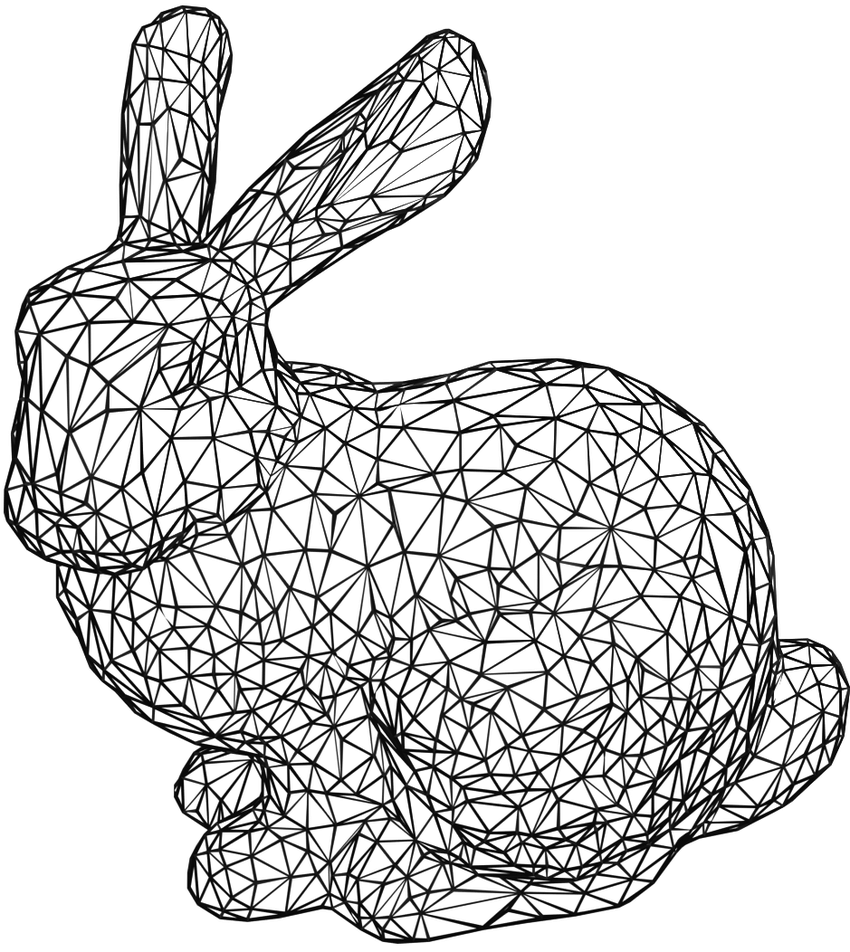
\includegraphics[width=0.5\textwidth]{images/stanford_bunny.png}
    \caption{Discretised bunny, taken from: \cite{discretebunny}}
    \label{fig:discretebunny}
\end{figure}

Intersection tests can be extended to complex object meshes very simply via efficient triangle intersection algorithms. The most common is the Möller–Trumbore algorithm \cite{trumboreintersection}. This algorithm is efficient and doesn't require precomputation of the triangle's plane equation.

E.g. for a mesh composed of many triangles, we perform the following steps:

For each triangle in the mesh:
\begin{enumerate}
    \item Perform the triangle intersection test.
    \item If an intersection is found, store the intersection point and distance.
\end{enumerate}

After testing all triangles, return the closest intersection point (smallest positive \(t\)). This will be where we will do our bounces from.

\subsection{Placing Objects into the World}

In computer graphics, assembling a scene involves defining the objects within it and positioning them appropriately. Consider the classic demonstration scene, the \textit{Cornell Box}~\cite{cornellbox}, a standard test for rendering algorithms to showcase accurate light transport and shading.
In the previous sections, I have discussed how to test intersections with various geometric primitives. However, building a complex scene like the Cornell Box requires a systematic way to place and manipulate these objects in three-dimensional space. We can do this via Matrices.

Matrices are fundamental tools in linear algebra that we can use to represent and compute transformations in space efficiently. We can represent operations such as:

\begin{itemize}
    \item \textbf{Translation}, moving an object by a certain distance along the axes.
    \item \textbf{Rotation}, turning an object around an axis.
    \item \textbf{Scaling}, resizing an object by stretching or compressing it along an axis.
\end{itemize}

We can then put these operations into mathematical objects that can be easily combined and applied to points and vectors in 3D space (and computed quickly on a GPU \cite{gpumatrixmultiplication}).

In our path tracer we can view a point or vector as a column vector (a matrix of N $\times$ 1):
\[
    \mathbf{v} = \begin{bmatrix} x \\ y \\ z \end{bmatrix}
\]
Transforming this vector involves multiplying it by a transformation matrix:
\[
    \mathbf{v}' = \mathbf{M} \mathbf{v}
\]
where \(\mathbf{v}'\) is the transformed vector and \(\mathbf{M}\) is the transformation matrix.
If we apply the transformation matrix to all points in our object, we have successfully transformed our object.

\subsubsection{Translation}

We will start with translation. In 3D space, we can represent a translation as a vector $\mathbf{d} = (d_x, d_y, d_z)$. Applying this translation to a point $\mathbf{p} = (x, y, z)$ is straightforward:

$$ \mathbf{p}' = \mathbf{p} + \mathbf{d} = \begin{bmatrix}
        x + d_x \\ y + d_y \\ z + d_z
    \end{bmatrix} $$

However, this addition operation \textit{cannot} be represented as a matrix multiplication with 3D vectors (due to it breaking the laws of linearity, see \autoref{sec:appendix-derivations-linear}). This is problematic as we want to unify all our transformations (translation, rotation, and scaling) into a single matrix operation (this is much more efficient).
To solve this, we introduce homogeneous coordinates. By adding a fourth component to our vectors (usually set to 1 for points and 0 for directions), we can represent translation as a 4x4 matrix multiplication:

In homogeneous coordinates, a point becomes:

\[
    \mathbf{v}_h = \begin{pmatrix} x \\ y \\ z \\ 1 \end{pmatrix}
\]

A translation matrix in homogeneous coordinates is:

\[
    \mathbf{T} = \begin{bmatrix}
        1 & 0 & 0 & d_x \\
        0 & 1 & 0 & d_y \\
        0 & 0 & 1 & d_z \\
        0 & 0 & 0 & 1   \\
    \end{bmatrix}
\]

The transformation is then applied via:

\[
    \begin{bmatrix}  1 & 0 & 0 & {T_x} \\ 0 & 1 & 0 & {T_y} \\ 0 & 0 & 1 & {T_z} \\ 0 & 0 & 0 & 1 \end{bmatrix} \cdot \begin{pmatrix} x \\ y \\ z \\ 1 \end{pmatrix} = \begin{pmatrix} x + {T_x} \\ y + {T_y} \\ z + {T_z} \\ 1 \end{pmatrix}
\]

Adding an extra dimension to our vectors and matrices allows us to represent all affine transformations, including translation, with 4$\times$4 matrices. Though we primarily use 3$\times$3 matrices for rotation and scaling in our renderer, working with homogeneous coordinates and 4$\times$4 matrices becomes essential for incorporating translation and perspective transformations.


\subsubsection{Scaling}

Scaling \textit{is} a linear transformation which means that it can be represented using a 3$\times$3 matrix, however as we would like all our transformations to multiply with each other we add a 4th scaling value of 1.

\[
    \begin{bmatrix}
        {S_1} & 0     & 0     & 0 \\
        0     & {S_2} & 0     & 0 \\
        0     & 0     & {S_3} & 0 \\
        0     & 0     & 0     & 1
    \end{bmatrix} \cdot
    \begin{pmatrix} x \\ y \\ z \\ 1 \end{pmatrix} =
    \begin{pmatrix} {S_x} \cdot x \\ {S_y} \cdot y \\ {S_z} \cdot z \\ 1 \end{pmatrix}
\]

where \( S_x \), \( S_y \), and \( S_z \) are the scaling factors along the \( x \), \( y \), and \( z \) axes, respectively.

\subsubsection{Rotation}

Rotation can also be represented using a 3$\times$3 matrix, but again, in practice they are represented as 4$\times$4 matrices.
Rotations in 3D are specified with an angle (in radians) and a rotation axis, with which you rotate the object around.

\paragraph{Rotation Around the X-axis}

Rotating a point around the \(x\)-axis by an angle \(\theta\):
\[
    \mathbf{R}_x(\theta) = \begin{bmatrix}
        1 & 0           & 0            & 0 \\
        0 & \cos \theta & -\sin \theta & 0 \\
        0 & \sin \theta & \cos \theta  & 0 \\
        0 & 0           & 0            & 1 \\
    \end{bmatrix}
\]

\paragraph{Rotation Around the Y-axis}
Rotating a point around the \(y\)-axis by an angle \(\theta\):
\[
    \mathbf{R}_y(\theta) = \begin{bmatrix}
        \cos \theta  & 0 & \sin \theta & 0 \\
        0            & 1 & 0           & 0 \\
        -\sin \theta & 0 & \cos \theta & 0 \\
        0            & 0 & 0           & 1 \\
    \end{bmatrix}
\]

\paragraph{Rotation Around the Z-axis}

Rotating a point around the \(z\)-axis by an angle \(\theta\):
\[
    \mathbf{R}_z(\theta) = \begin{bmatrix}
        \cos \theta & -\sin \theta & 0 & 0 \\
        \sin \theta & \cos \theta  & 0 & 0 \\
        0           & 0            & 1 & 0 \\
        0           & 0            & 0 & 1 \\
    \end{bmatrix}
\]

If you are interested in how we can derive these rotation matrices, I have included it in \autoref{sec:appendix-derivations-rotation}.

These transformation matrices can be combined into a single matrix through multiplication, allowing us to apply multiple transformations in one operation. The order of multiplication is important, as matrix multiplication is not commutative. Typically, we combine transformations in the order of scale, then rotate, then translate.

I will demonstrate with an example, scale an object by 2 in all dimensions, rotate it 45° around the y-axis, and then translate it by (1, 2, 3), we would have:

\[
    \mathbf{M} =
    \begin{bmatrix}
        1 & 0 & 0 & 1 \\
        0 & 1 & 0 & 2 \\
        0 & 0 & 1 & 3 \\
        0 & 0 & 0 & 1
    \end{bmatrix} \cdot
    \begin{bmatrix}
        \cos 45°  & 0 & \sin 45° & 0 \\
        0         & 1 & 0        & 0 \\
        -\sin 45° & 0 & \cos 45° & 0 \\
        0         & 0 & 0        & 1
    \end{bmatrix} \cdot
    \begin{bmatrix}
        2 & 0 & 0 & 0 \\
        0 & 2 & 0 & 0 \\
        0 & 0 & 2 & 0 \\
        0 & 0 & 0 & 1
    \end{bmatrix}
\]
\[
    \mathbf{M} = \begin{bmatrix}
        1.41  & 0 & 1.41 & 1 \\
        0     & 2 & 0    & 2 \\
        -1.41 & 0 & 1.41 & 3 \\
        0     & 0 & 0    & 1
    \end{bmatrix}
\]

This combined matrix $\mathbf{M}$ can then be applied to all points in our object to achieve the desired transformation in a single step.

With this knowledge we can set up our cornell box scene:
\begin{figure}[H]
    \centering
    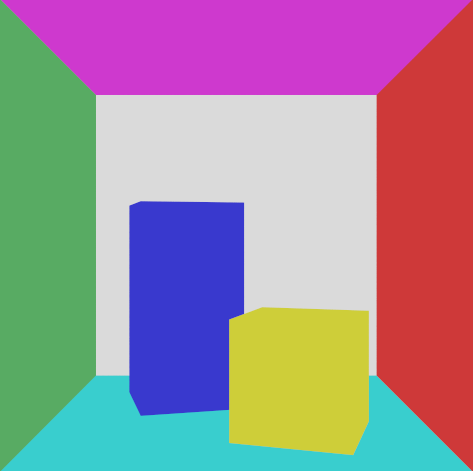
\includegraphics[width=0.5\textwidth]{images/artsy_rep/no_lighting_cornell.png}
    \caption{Cornell Box Objects}
    \label{fig:unlitcornell}
\end{figure}

\subsubsection{Model-View-Projection Matrix}
I need to mention an essential 3D graphics tool here, which will be useful to know later (\ref{sec:camera}). The Model-View-Projection (MVP) matrix transforms 3D objects from their local coordinate space to 2D screen coordinates. This transformation contains three stages:

\begin{description}
    \item[Model Matrix] The model matrix is composed of the transformations we've discussed (translation, rotation, and scaling) applied to an object to position it in the world.

    \item[View Matrix] The view matrix represents the camera's position and orientation in the world. It's essentially the inverse of the camera's transformation matrix, moving the world relative to the camera.

    \item[Projection Matrix] The projection matrix defines how 3D points in camera space are projected onto the 2D screen.

\end{description}

The MVP matrix is the product of these three matrices:
$MVP = Projection \cdot View \cdot Model $

We will not use the full MVP matrix in our path tracer. However, we have just made the Model Matrix for our objects, and we can use the inverse of the view matrix to transform rays from camera space to world space, then intersect these rays with objects in world space. The projection is handled implicitly by generating rays based on the camera's properties.

\paragraph{Mathematical intuition}
I described using these matrices to transform an object from a "space" to another "space" and I want to express this properly. The transformations we've discussed can instead be viewed as changes in the coordinate system or "space" in which we represent our objects. Each space is defined by a set of basis vectors, which are the fundamental directions that span that space. When we transform an object from one space to another, we're essentially changing the basis vectors used to describe the object's position and orientation. This added intuition should make understanding a transformed objects intersection code much easier to understand:

Let \(\mathbf{B} = [\mathbf{b}_1, \mathbf{b}_2, \mathbf{b}_3]\) be an orthonormal basis in the object's local space. A ray in world coordinates \(\mathbf{R}(t) = \mathbf{O} + t\mathbf{D}\) can be transformed into this basis using:

\[
    \mathbf{O}' = \mathbf{B}^{-1} (\mathbf{O} - \mathbf{P})
\]
\[
    \mathbf{D}' = \mathbf{B}^{-1} \mathbf{D}
\]

where \(\mathbf{P}\) is the object's position in world coordinates. Post intersection, the intersection point and normal can be transformed back into world space by:

\[
    \mathbf{P}_{\text{world}} = \mathbf{B} \mathbf{P}_{\text{local}} + \mathbf{P}
\]
\[
    \mathbf{N}_{\text{world}} = \mathbf{B} \mathbf{N}_{\text{local}}
\]

The advantage of this approach is that it allows us to define objects in their own local coordinate system, which is much more intuitive and easier to work with.

\subsection{Color and Shading Models}
\label{color_shading}
Having established our scene and implemented the ability to compute intersections between rays and objects, we must find some way to use this information to simulate how light works in the real world. This involves modelling how light behaves upon hitting different surfaces.

\paragraph{Light and Material Interaction}
The appearance of objects in a scene is influenced by how they interact with light. Light can be absorbed, reflected, or transmitted when it strikes a surface. The material properties of the surface govern these interactions.

In the initial implementation~\ref{fig:unlitcornell}, I simplified the shading process by assigning a static colour to each object upon ray intersection. In reality, a ray of light will take on the colour of a surface albedo due to a partial reflection of all the wavelengths of white light.

This ray may then propagate through the scene, interacting with other objects and accumulating colour contributions. The material properties dictate whether the light is absorbed, reflected, or refracted at each interaction point. For example, darker surfaces absorb more light and thus appear darker.

\subsubsection{Diffuse Reflection}
The first material I will cover is perfectly diffused as it is easy to understand. If a ray hits the surface, it will bounce randomly in any direction (with slightly less brightness). This ray will then hit something else, and so on, until it reaches a max recursion depth (at which point we can return black). This perfectly diffuse material is not the most realistic but is a good starting point, used by many of the first raytracing papers \cite{Whitted1980}. Here is what this method would look like with global illumination:

\begin{figure}[H]
    \centering
    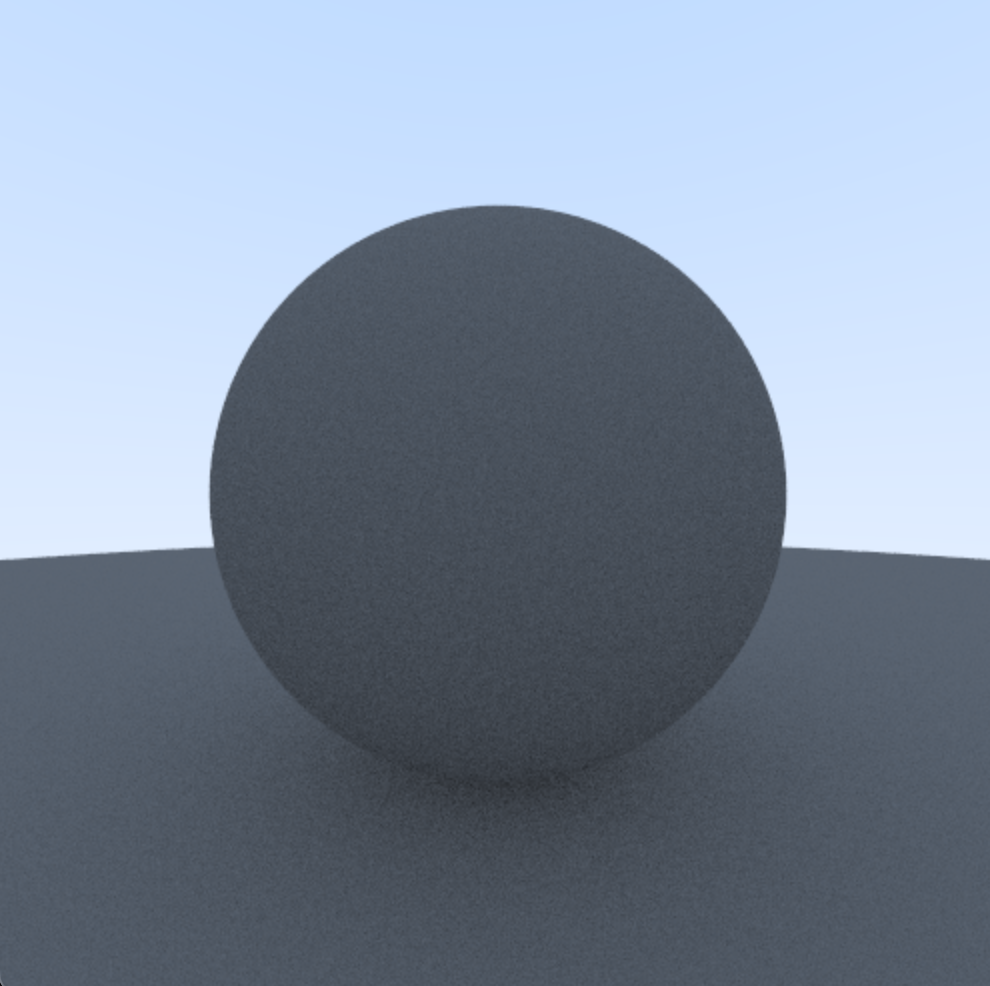
\includegraphics[width=0.5\textwidth]{images/lambertian/uniform_diffuse.png}
    \caption{Perfectly diffuse material}
    \label{fig:perfdiffmat}
\end{figure}

Though this simple method yields good results, in reality, the Lambert Cosine Law comes into effect. This law states that the intensity of reflected light depends on the angle's cosine between the incoming light direction and the surface normal. Therefore, we need to adjust the power of reflection according to this principle.

The intensity \(I\) of the reflected light is proportional to the cosine of the angle \(\theta\) between the light direction \(\mathbf{L}\) and the surface normal \(\mathbf{N}\):
\[
    I = I_0 \cdot \max(\mathbf{L} \cdot \mathbf{N}, 0)
\]
where \(I_0\) is the intensity of the incoming light. This cosine dependency ensures that light hitting the surface at a shallow angle contributes less to the reflected intensity.
This type of material is called a Lambertian:

\begin{figure}[H]
    \centering
    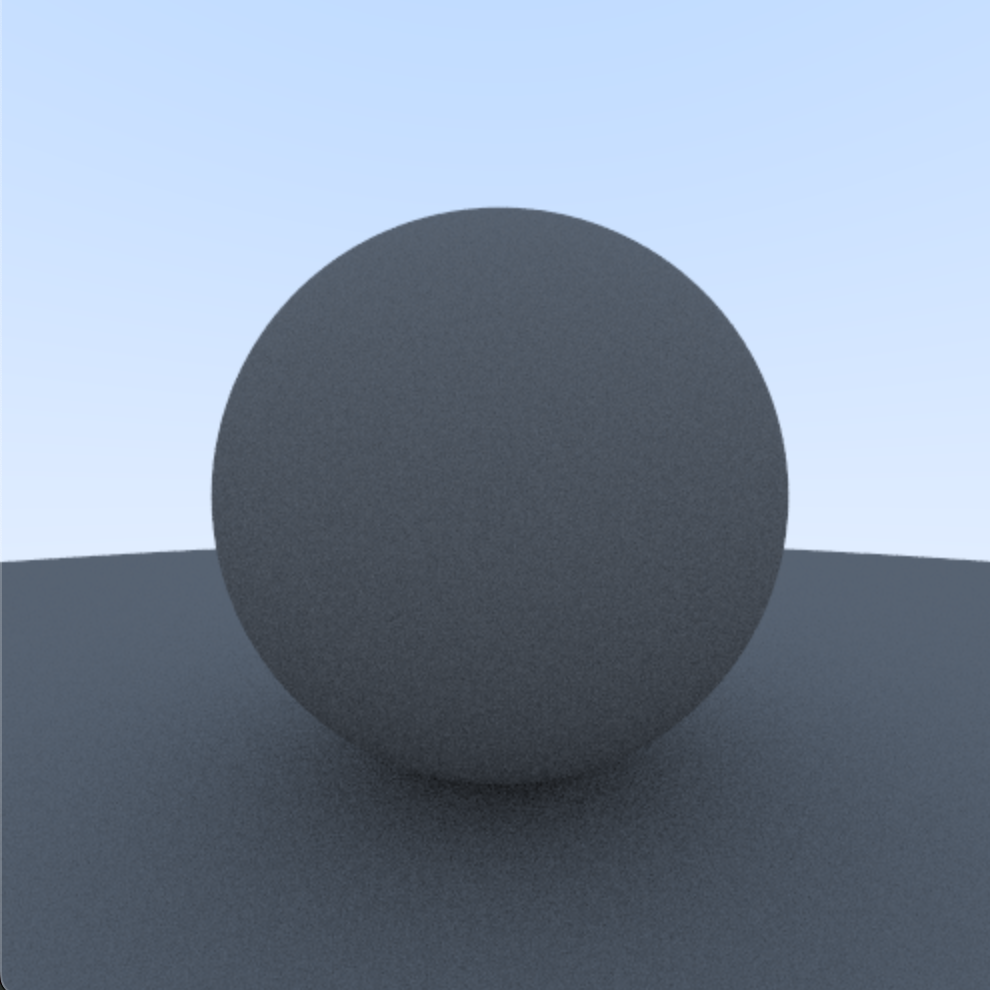
\includegraphics[width=0.5\textwidth]{images/lambertian/lambertian_diffuse.png}
    \caption{Lambertian diffuse material}
    \label{fig:lambdiffmat}
\end{figure}

If you look closely you will notice that the shadows are much more pronounced (and accurate).

\subsubsection{Specular Reflection}
Specular reflection occurs on shiny surfaces where light is reflected in a specific direction. In a perfect mirror we want to "reflect" the ray according to its angle of incidence, instead of randomly in any direction.
The reflection vector \(\mathbf{R}\) is computed as:
\[
    \mathbf{R} = \mathbf{L} - 2(\mathbf{L} \cdot \mathbf{N})\mathbf{N}
\]
The intensity of the reflected light depends on the angle between the reflection vector \(\mathbf{R}\) and the view direction \(\mathbf{V}\):
\[
    I = I_0 \cdot \max(\mathbf{V} \cdot \mathbf{R}, 0)^n
\]
where \(n\) is the shininess coefficient, determining the sharpness of the reflection.

\begin{figure}[H]
    \centering
    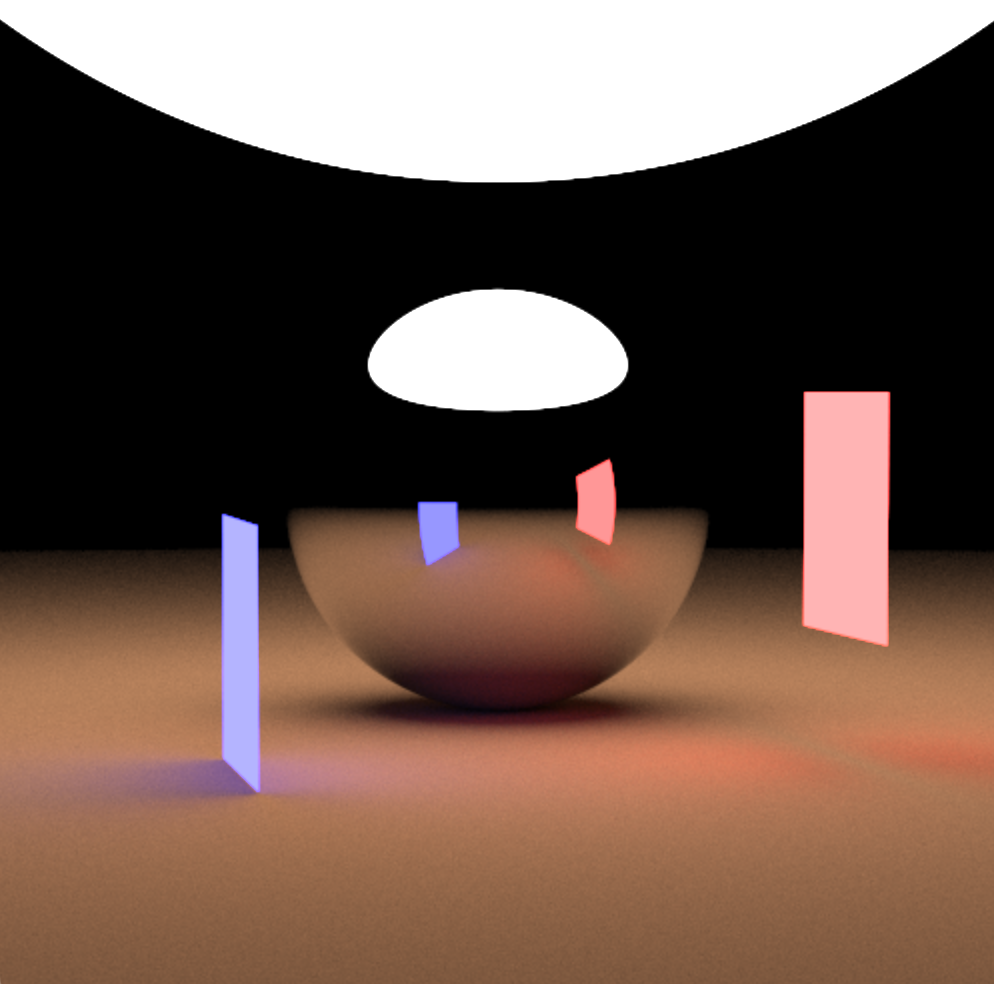
\includegraphics[width=0.5\textwidth]{images/artsy_rep/specular_sphere.png}
    \caption{Specular material}
    \label{fig:specmat}
\end{figure}

Notice the bending of the lights in the spheres reflection. This type of image is why path tracers really blow my mind, think about how little we have had to do to arrive at an image which has such realistic lighting!

\section{Camera Dynamics}
\label{sec:camera}

Cameras in path tracing simulate the human eye or a physical camera, capturing scenes from a specific viewpoint. The camera's parameters, such as position, orientation, and field of view, allowing us to play with the composition and visual realism of the final image.

\paragraph{Basis Vectors and Camera Orientation}
To accurately orient the camera in a scene, we create a local coordinate system using three orthonormal basis vectors: \(\mathbf{u}\), \(\mathbf{v}\), and \(\mathbf{w}\). These vectors allow us to easily project a viewport grid onto the physical pixels of our image. The vectors also allow us to move the camera's orientation and not have to worry about projection complexities.

The camera's orientation is specified by the following vectors:

\(\mathbf{w}\): This vector points from the camera position towards the look-at point, essentially defining the view direction. It is calculated as:
\[
    \mathbf{w} = \frac{\mathbf{C} - \mathbf{L}}{\|\mathbf{C} - \mathbf{L}\|}
\]
where \(\mathbf{C}\) represents the camera's position, and \(\mathbf{L}\) is the focal point of our image.

\(\mathbf{u}\): This vector points to the camera's right and is derived from the cross product of the global up vector \(\mathbf{v}_{\text{up}}\) and \(\mathbf{w}\):
\[
    \mathbf{u} = \frac{\mathbf{v}_{\text{up}} \times \mathbf{w}}{\|\mathbf{v}_{\text{up}} \times \mathbf{w}\|}
\]

\(\mathbf{v}\): This vector points upward in the camera's local space, calculated by the cross product of \(\mathbf{w}\) and \(\mathbf{u}\):
\[
    \mathbf{v} = \mathbf{w} \times \mathbf{u}
\]

These vectors form a right-handed coordinate system, defining the camera's spatial alignment and enabling intuitive manipulation of the camera's orientation in the scene.

\subsection{Camera Ray Generation}
We currently have the ability to send rays throughout a 3D scene, but a screen is a 2D plane so we must project our data into it. In path tracing this is achieved by calculating a viewports dimensions from our camera's basis vectors, alongside pixel information from our applications window (I am using the library GLFW to manage the window). As mentioned previously, a different method of doing this is using the Projection matrix (computed from our camera's parameters).

To accurately simulate the projection of rays from the camera through each pixel on the image plane, we need to establish a relationship between the camera's properties, the viewport, and the pixels in our final image. Let's break this down step by step:

We start with a camera defined by its position $\mathbf{C}$, and orthonormal basis vectors $\mathbf{u}$, $\mathbf{v}$, and $\mathbf{w}$, representing the camera's local coordinate system.

The viewport represents the camera's view of the scene. Its dimensions are determined by the vertical field of view (FOV) and the aspect ratio of the rendered image:

$$ \text{viewportHeight} = 2 \cdot \tan\left(\frac{\text{vertFOV}}{2}\right) \cdot \text{focalLength}
    \ $$
$$ \text{viewportWidth} = \text{viewportHeight} \cdot \frac{\text{imageWidth}}{\text{imageHeight}}
    \ $$

This ensures that the viewport's proportions match the final image, preventing distortion.

We define vectors representing the viewport's extent in the camera's local coordinate system:

$$ \text{viewportU} = \text{viewportWidth} \cdot \mathbf{u}
    \ $$
$$ \text{viewportV} = \text{viewportHeight} \cdot \mathbf{v}
    \ $$

To map our image pixels to viewport positions, we calculate the spacing between pixels:

$$ \text{pixelDeltaU} = \frac{\text{viewportU}}{\text{imageWidth}}
    \ $$
$$ \text{pixelDeltaV} = \frac{\text{viewportV}}{\text{imageHeight}}
    \ $$

We then position the viewport in the camera's local space:

$$ \text{viewportUpperLeft} = \mathbf{C} - (\text{focalLength} \cdot \mathbf{w}) - \frac{\text{viewportU}}{2} - \frac{\text{viewportV}}{2}
    \ $$

This places the viewport at the focal length from the camera, centered in the camera's view.

Finally, we can calculate the position of each pixel in the viewport:

$$ \text{pixelTL} = \text{viewportUpperLeft} + 0.5 \cdot (\text{pixelDeltaU} + \text{pixelDeltaV})
    \ $$

Other pixels are positioned by adding multiples of $\text{pixelDeltaU}$ and $\text{pixelDeltaV}$ to $\text{pixelTL}$.

By following these steps, we have created a direct mapping between each pixel in our image and a corresponding point in the camera's viewport. The ray direction for each pixel can then be calculated as the vector from the camera position $\mathbf{C}$ to the pixel's position in the viewport.


\paragraph{Field Of View} The camera's field of view (FOV) determines how much of the scene is visible through the viewport, affecting the perceived scale and perspective, as scene in our $\text{viewportHeight}$ equation.
These parameters allow us to replicate how a real-world camera captures a scene, but we can also manipulate the FOV to get some artistic effects:

\begin{figure}[H]
    \centering
    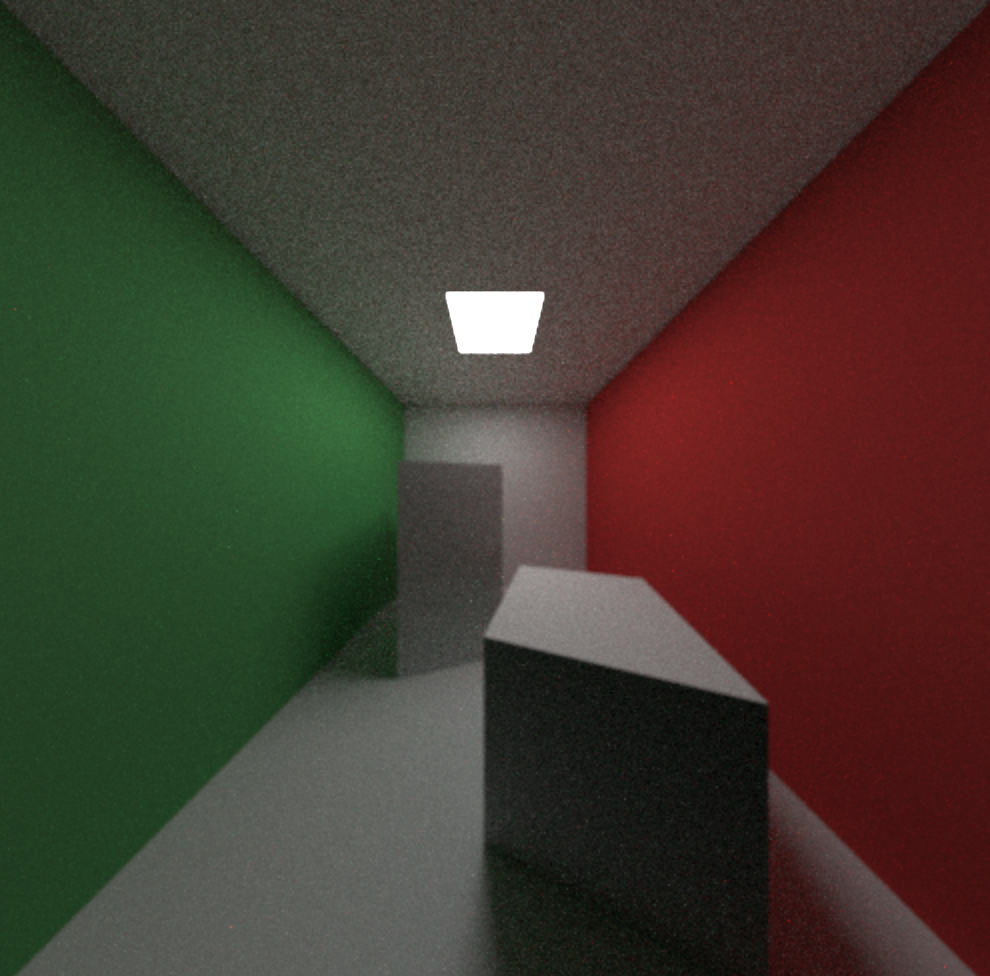
\includegraphics[width=0.5\textwidth]{images/artsy_rep/highFOV_cornell.png}
    \caption{Cornell box rendered with high FOV}
    \label{fig:highFOVBox}
\end{figure}

The geometry of the Cornell box has remained identical, however we have achieved an effective emulation of a "Fish-eye" lens.

\subsection{Camera Aliasing}
This camera model we just established is fundamental to the ray tracing process. It generates rays from the camera's origin, passing through each pixel on the image plane, and now stores this information on our window. However, lets look closely at an image I generated of two spheres (pink and green) intersecting:

\begin{figure}[H]
    \centering
    
\includegraphics[width=0.5\textwidth]{images/aliasing/no-aliasing.png}
    \caption{Aliased interactions}
    \label{fig:aliasedintersection}
\end{figure}

This does not very spherical to me! A crucial challenge we have in rendering involves aliased edges, in which a pixel's ray either hits an object or misses it entirely. This binary decision creates very jagged edges, as briefly referenced in Figure \ref{fig:raysphereintersection}.

To address this, we employ anti-aliasing techniques. There are many many ways techniques with lots of acronyms (FXAA, SMAA, MSAA, TXAA etc.), but I will tackle Super Sampling Anti-Aliasing (SSAA). SSAA is one of the most effective method, in which \textit{multiple} samples per pixel are taken, and their colors are averaged together. By randomly choosing a direction within the pixel, we manage smooth out the transitions and enhance image quality:

\begin{figure}[H]
    \centering
    
\includegraphics[width=0.5\textwidth]{images/aliasing/aliased.png}
    \caption{SSAA intersections}
    \label{fig:antialiasedintersection}
\end{figure}

As we can see SSAA significantly reduces aliasing artifacts, producing more realistic and visually appealing results by blurring the sharp transitions at object boundaries.
This is not a solved issue however, as SSAA is incredibly expensive to perform, if we want to perform 16xSSAA (16 samples per pixel) then our computation time will be proportionally longer (16x longer!). The next section will focus on how we can get more out of each sample we take.

\section{Acceleration Structures UNFINISHED (ONLY IN CODE)}
\label{sec:acceleration-structures}
\subsection{Bounding Volume Hierarchies (BVH)}
\subsubsection{Overview of BVH}
\subsubsection{Technical Implementation}
\subsubsection{Algorithmic Analysis}

\pagebreak
\section{Monte Carlo Methods for Ray Tracing}
\label{sec:monte-carlo}

This section focuses on enhancing the efficiency and quality of our path tracer through the application of advanced probabilistic techniques. While we will not introduce new visual elements, these methods will significantly improve our ray tracer's performance and convergence rate.

\subsection{Improved Random Sampling}
In our previous Super Sampling Anti-Aliasing (SSAA) implementation, we employed a simple random ray generation strategy for each pixel. This approach is very effective; however, it suffers from high variance, leading to slower convergence and potentially noisy results. To address this limitation, I will introduce stratified sampling.

Stratified sampling involves dividing the sampling domain into non-overlapping regions, or strata, and sampling from within each stratum. It can help to imagine placing a 2x2 square over each pixel and then ensuring you sample from each quadrant. If we compare this to random sampling 4 times, it makes intuitive sense that we would get more information (on average).
The stratified approach ensures a more uniform distribution of samples across the pixel, which can be expressed mathematically as follows:

Simple Random Sampling:

In this method, we take $n$ independent samples $X_1, X_2, ..., X_n$ randomly from the entire domain. The variance of the sample mean $\hat{f}$ is given by:

\[
    \text{Var}(\hat{f}) = \frac{\sigma^2}{n}
\]

Where:
$\hat{f}$ is the estimated mean of the function and $\sigma^2$ is the variance of the function $f(x)$ over its entire domain.

Stratified Sampling:

In stratified sampling, we divide the domain into $k$ strata (sub-regions) and sample within each stratum. Assuming equal sampling in each stratum, the variance of the stratified sample mean $\hat{f}_s$ is:

\[
    \text{Var}(\hat{f}_s) = \frac{1}{n} \left( \sigma^2 - \frac{1}{k} \sum_{i=1}^k \sigma_i^2 \right)
\]

Where $\sigma_i^2$ is the variance within the $i$-th stratum, $k$ is the number of strata and $n$ is the total number of samples.

This formula is derived by examining the variance over the entire domain and adjusting for the reduced variance within each stratum. Here’s why each term appears:

\begin{enumerate}
    \item Total Variance $\sigma^2$: This represents the overall variability of the function across the entire domain without any stratification. It is the "baseline" amount of variance we would have if we did not use stratified sampling.

    \item Reducing Variance with Strata: When we divide the domain into $k$ strata, each one is designed to be more homogeneous than the domain as a whole. As a result, the variance within each stratum, $\sigma_i^2$, is expected to be smaller than the total variance $\sigma^2$. The term $\frac{1}{k} \sum_{i=1}^k \sigma_i^2$ represents the average of these reduced variances across all $k$ strata.

    \item Variance Reduction Effect: The formula subtracts $\frac{1}{k} \sum_{i=1}^k \sigma_i^2$ from $\sigma^2$ because the stratified approach lowers the overall variance by the average of these within-strata variances. So, we essentially say, "Start with the total variance, but then subtract out the portion that stratification has reduced."

    \item Normalization by Total Samples $n$: Finally, we divide by $n$ because the variance of the mean over $n$ samples scales down as more samples are taken \footnote{The central limit theorem states that the distribution of sample means tends to approximate a normal distribution as the sample size $n$ increases, regardless of the distribution of the original data. Additionally, the variability (or variance) of the sample mean decreases with more samples by a factor of $\frac{1}{n}$. This is why dividing by $n$ is necessary; as $n$ grows, the variance of our mean estimate $\hat{f}$ decreases, leading to a smoother, more accurate result.}.

\end{enumerate}

To compare these methods more concretely, let's consider an example with 16 samples arranged in a 4x4 grid ($n = 16$, $k = 16$):

Simple Random Sampling Variance:
\[
    \text{Var}(\hat{f}) = \frac{\sigma^2}{16} = 0.0625\sigma^2
\]

Stratified Sampling Variance: Assuming the variance within each stratum is equal and denoted by $\sigma^2_i$, the stratified sampling variance becomes:

\[
    \text{Var}(\hat{f}_s) = \frac{1}{16} \left( \sigma^2 - \frac{1}{16} \sum_{i=1}^{16} \sigma_i^2 \right)
\]

We can then assume $\sigma_i^2 \approx \frac{\sigma^2}{16}$ based on the reasonable approximation that each stratum's variance is proportional to the size of the stratum relative to the whole.
\[
    \text{Var}(\hat{f}_s)
    = \frac{1}{16} \left( \sigma^2 - \frac{1}{16} \cdot 16 \cdot \frac{\sigma^2}{16} \right)
    = \frac{1}{16} \left( \frac{15}{16} \sigma^2 \right)
    = \frac{15}{256}\sigma^2 \approx 0.0586\sigma^2
\]

Comparing the results:
\begin{enumerate}
    \item[] Simple Random Sampling Variance: $0.0625\sigma^2$
    \item[] Stratified Sampling Variance: $0.0586\sigma^2$
\end{enumerate}

We can see that even in this simplified model, stratified sampling reduces the variance compared to simple random sampling. Unfortunately, we cannot declare that we should now have one million strata for the best results as the benefits plateau with increasing strata. The variance reduction depends on how much the function varies within each stratum. When too many strata exist, each stratum becomes tiny, capturing little additional information about the function's overall behaviour. Consequently, the average variance within each stratum, $\sigma_i^2$, approaches zero, which makes the formula $\text{Var}(\hat{f}_s) = \frac{1}{n} \left( \sigma^2 - \frac{1}{k} \sum_{i=1}^k \sigma_i^2 \right)$ asymptotically approach $\frac{\sigma^2}{n}$, essentially the same as simple random sampling.

Figure \ref{fig:strat_comparison} provides a visual comparison between random sampling and stratified sampling, both using 64 rays per pixel.

\begin{figure}[H]
    \centering
    \begin{subfigure}[b]{0.45\textwidth}
        \centering
        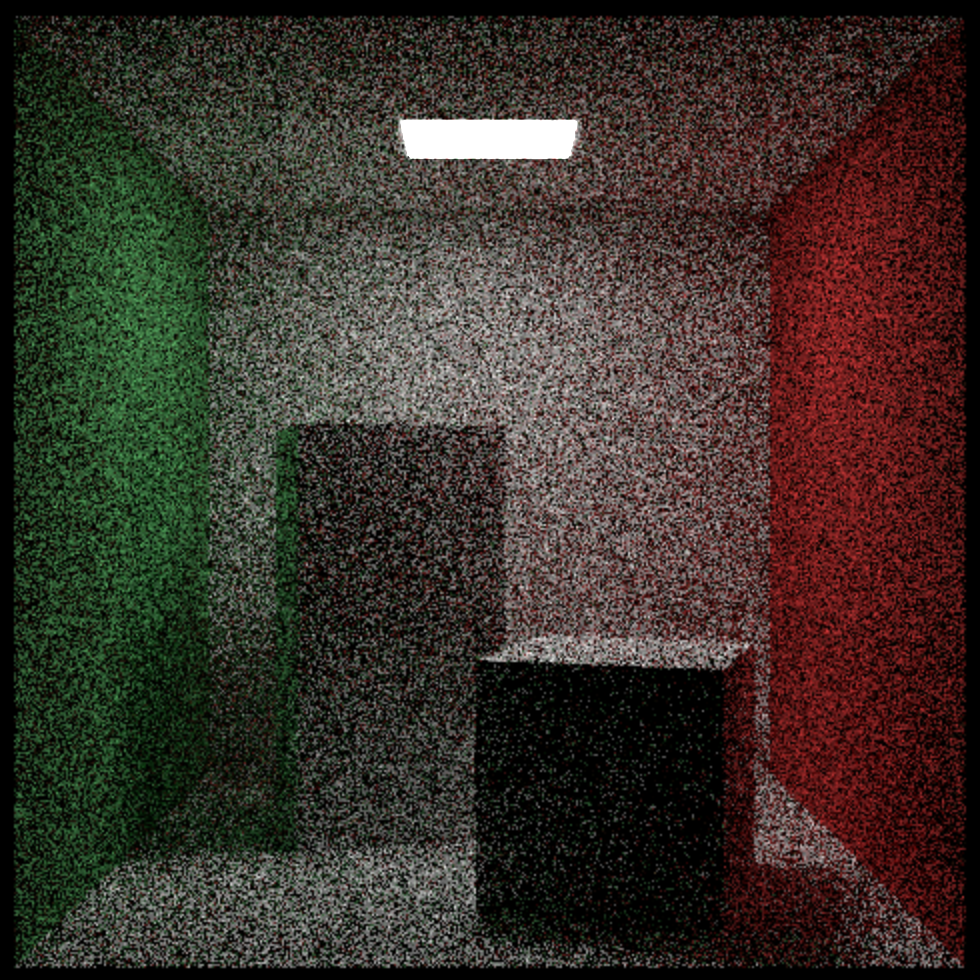
\includegraphics[width=\textwidth]{images/strat_vs_non/1sam64tim.png}
        \caption{Rendered image using random sampling}
        \label{fig:randomsamplesno_strat}
    \end{subfigure}
    \hfill
    \begin{subfigure}[b]{0.45\textwidth}
        \centering
        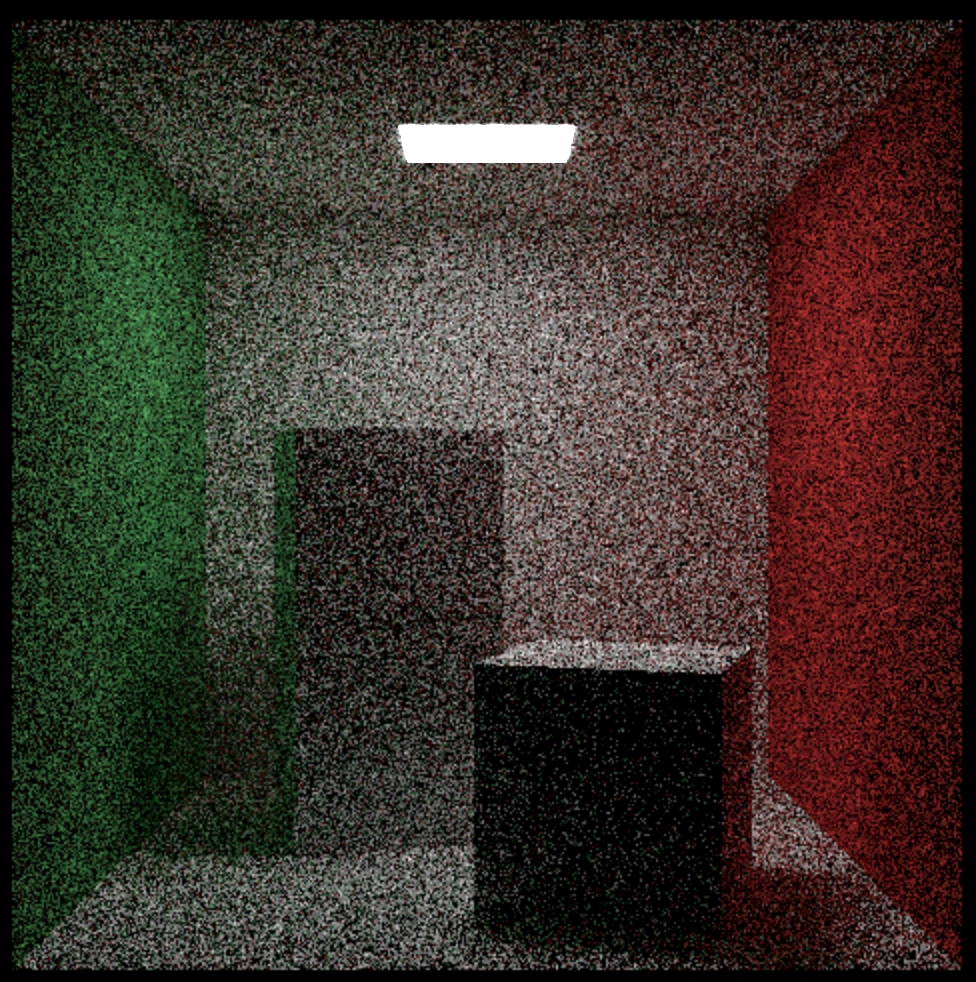
\includegraphics[width=\textwidth]{images/strat_vs_non/64sam1tim.png}
        \caption{Rendered image using stratified sampling}
        \label{fig:stratified_sampling}
    \end{subfigure}
    \caption{Comparison of image rendered with 64 rays per pixel}
    \label{fig:strat_comparison}
\end{figure}
The benefits of stratified sampling are most pronounced in areas with high-frequency details or sharp transitions, such as the edges of objects. This may be hard to see with such a simple scene. However, if you look in the very centre of the image, you should notice that you can see that the stratified sampling approach (Figure \ref{fig:stratified_sampling}) produces more defined edges for the boxes against the background compared to the random sampling method (Figure \ref{fig:randomsamplesno_strat}). This improved edge definition results from the more uniform distribution of samples across each pixel, better capturing the transition between object boundaries and their surroundings.

\subsection{Importance Sampling}

\paragraph{The Problem of Noise and Slow Convergence} The current theory allows for an elegant path tracer capable of producing visually realistic images. However, it has some very fundamental problems. To illustrate these, let us look at our Cornell box scene with one ray fired per pixel (so no SSAA) and a maximum bounce of 1000 (much higher than 99\% of rays will get to).

\begin{figure}[H]
    \centering
    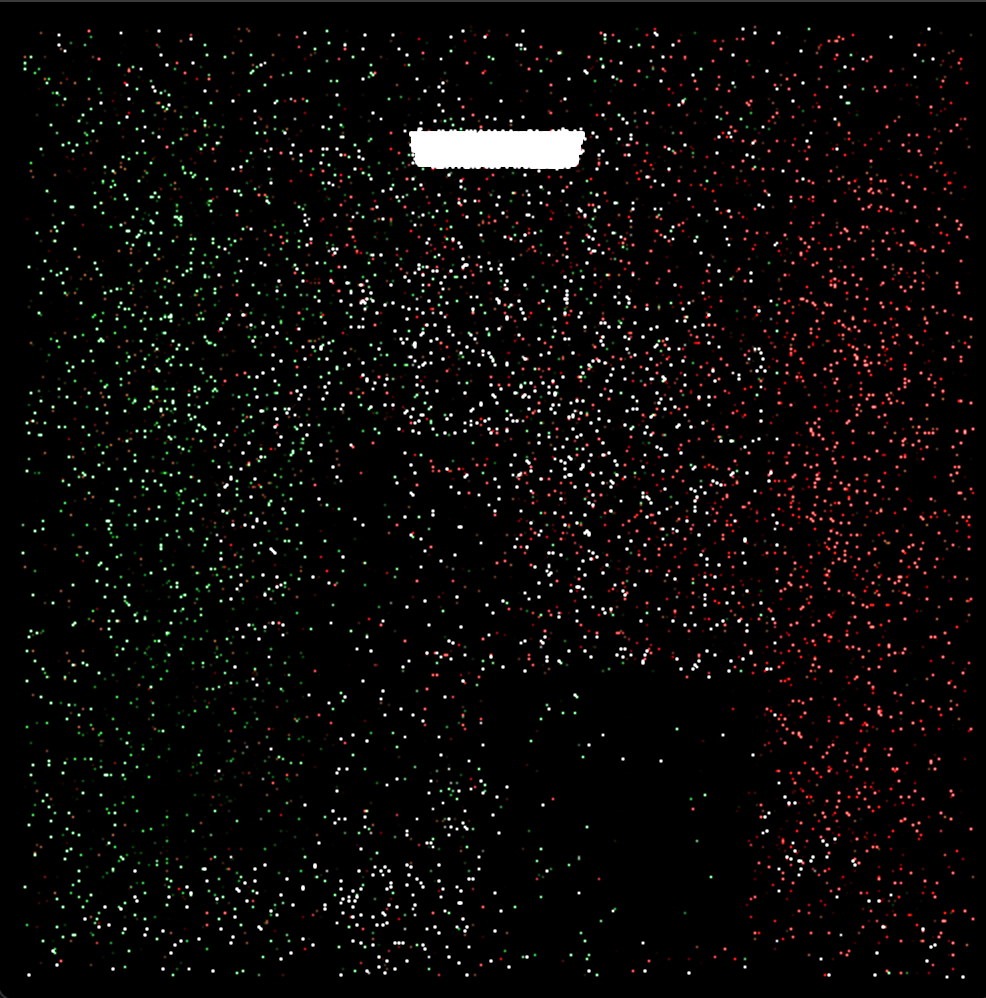
\includegraphics[width=0.5\textwidth]{images/one_samp/random_sample.png}
    \caption{One Sample Cornell box}
    \label{fig:onesampcornell}
\end{figure}

As we can see most rays bounce around, never hit a light and then bounce back out of the box into the darkness. Because of this the vast majority of our rays contribute no color to our scene.

\paragraph{Biasing Rays Towards Light Sources}

We can bias our ray sampling towards light sources to address this issue. A naive approach is to fire our rays into the scene and then, at an intersection, check if the light is visible and send the ray to a random point on the light. This yields something like this:

\begin{figure}[H]
    \centering
    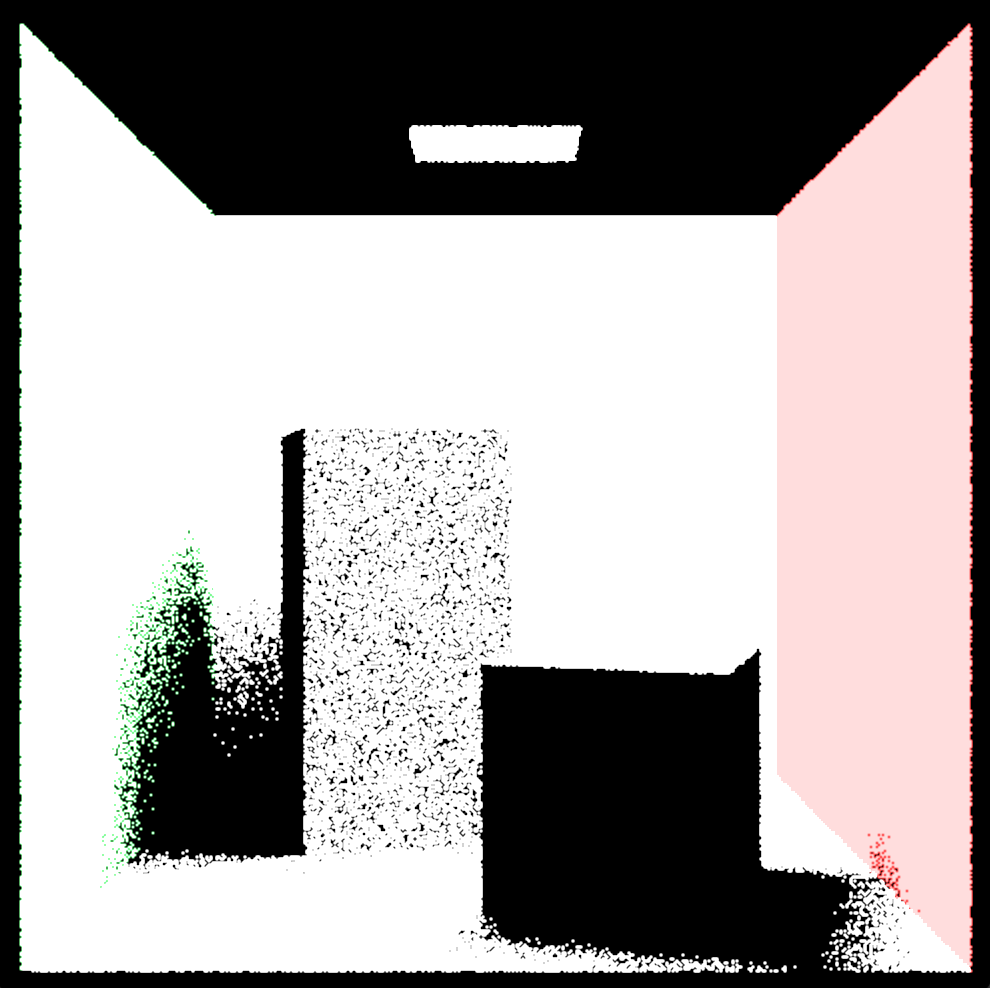
\includegraphics[width=0.5\textwidth]{images/one_samp/towards_light_no_pdf.png}
    \caption{Sampling towards a light}
    \label{fig:onesampimportancenopdf}
\end{figure}

It is clear now that we have accrued the exact opposite problem! Biasing all rays towards light sources introduces a new problem: the rendered image becomes excessively bright. This occurs because we are now oversampling the light sources without adequately accounting for this bias in our estimator. Interestingly, this technique gives us a much clearer idea of the scene, indicating we are on the right track.

\subsubsection{Correcting Bias}


In our ideal world, we would be able to do the same thing we just did, but for all the rays that go directly to the light, we turn the contribution to the final image down, and for each ray that has not directly hit a light (quite unlikely) we turn their contribution way up.

We need two mathematical tools for this:
\begin{enumerate}
    \item A method of generating a biased random direction (so that we can sample towards our light)
    \item A method that, when given a biased random direction, tells us how likely it was to be generated (so that we can turn down/up its intensity by how much it'll be sampled)
\end{enumerate}

We already have the former; pick a random point on the light and send a ray in that direction. However, for the latter we need to use a tool from statistics, the Probability Density Function (PDF).

\paragraph{PDFs} To understand Probability Density Functions (PDFs), let's start with a familiar concept: histograms. In the context of path tracing, imagine we create a histogram of the directions of rays bouncing off a surface. This histogram divides the hemisphere above the surface into sections and shows the frequency of rays in each section.

As we increase our sample size (i.e., trace more paths), the frequency in each section grows, but the overall distribution of ray directions becomes more defined. If we normalize the y-axis of our histogram to show the fraction of total rays in each section instead of raw counts, we create a discrete density function:

$$
    \text{Density of section } i = \frac{\text{Number of rays in section } i}{\text{Total number of rays}}
$$

To move from this discrete representation to a continuous one, we can consider what happens as we increase the number of sections indefinitely while narrowing their solid angle. In the limit, we arrive at a continuous density function:

$$
    \text{Density at direction } \omega = \lim_{\Delta \omega \to 0} \frac{\text{Fraction of rays between } \omega \text{ and } \omega + \Delta \omega}{\Delta \omega}
$$

This continuous density function is our Probability Density Function (PDF). While the probability of a ray having any exact direction is zero (there are infinitely many possible directions), we can use the PDF to find the probability of a ray falling within any range of directions by integrating the PDF over that range:

$$
    P(\omega_1 \leq \text{direction} \leq \omega_2) = \int_{\omega_1}^{\omega_2} \text{PDF}(\omega) \, d\omega
$$

In path tracing, PDFs are crucial for importance sampling. They allow us to sample ray directions non-uniformly, focusing on directions that are more likely to contribute significantly to the final image (such as towards light sources), while still maintaining an unbiased estimate by weighting the contributions of these biased samples. For our light-biased sampling strategy, the PDF will have higher values for directions towards the light and lower values elsewhere.

\paragraph{Deriving our Light's PDF}

To understand how we arrive at the PDF for our light source, let us consider the geometry of the situation. Imagine we have a point on a surface in our scene, and we want to sample the light source from this point. In this case, the light source is a quad (a rectangular area light) on the ceiling of our Cornell box.

\begin{figure}[H]
    \centering
    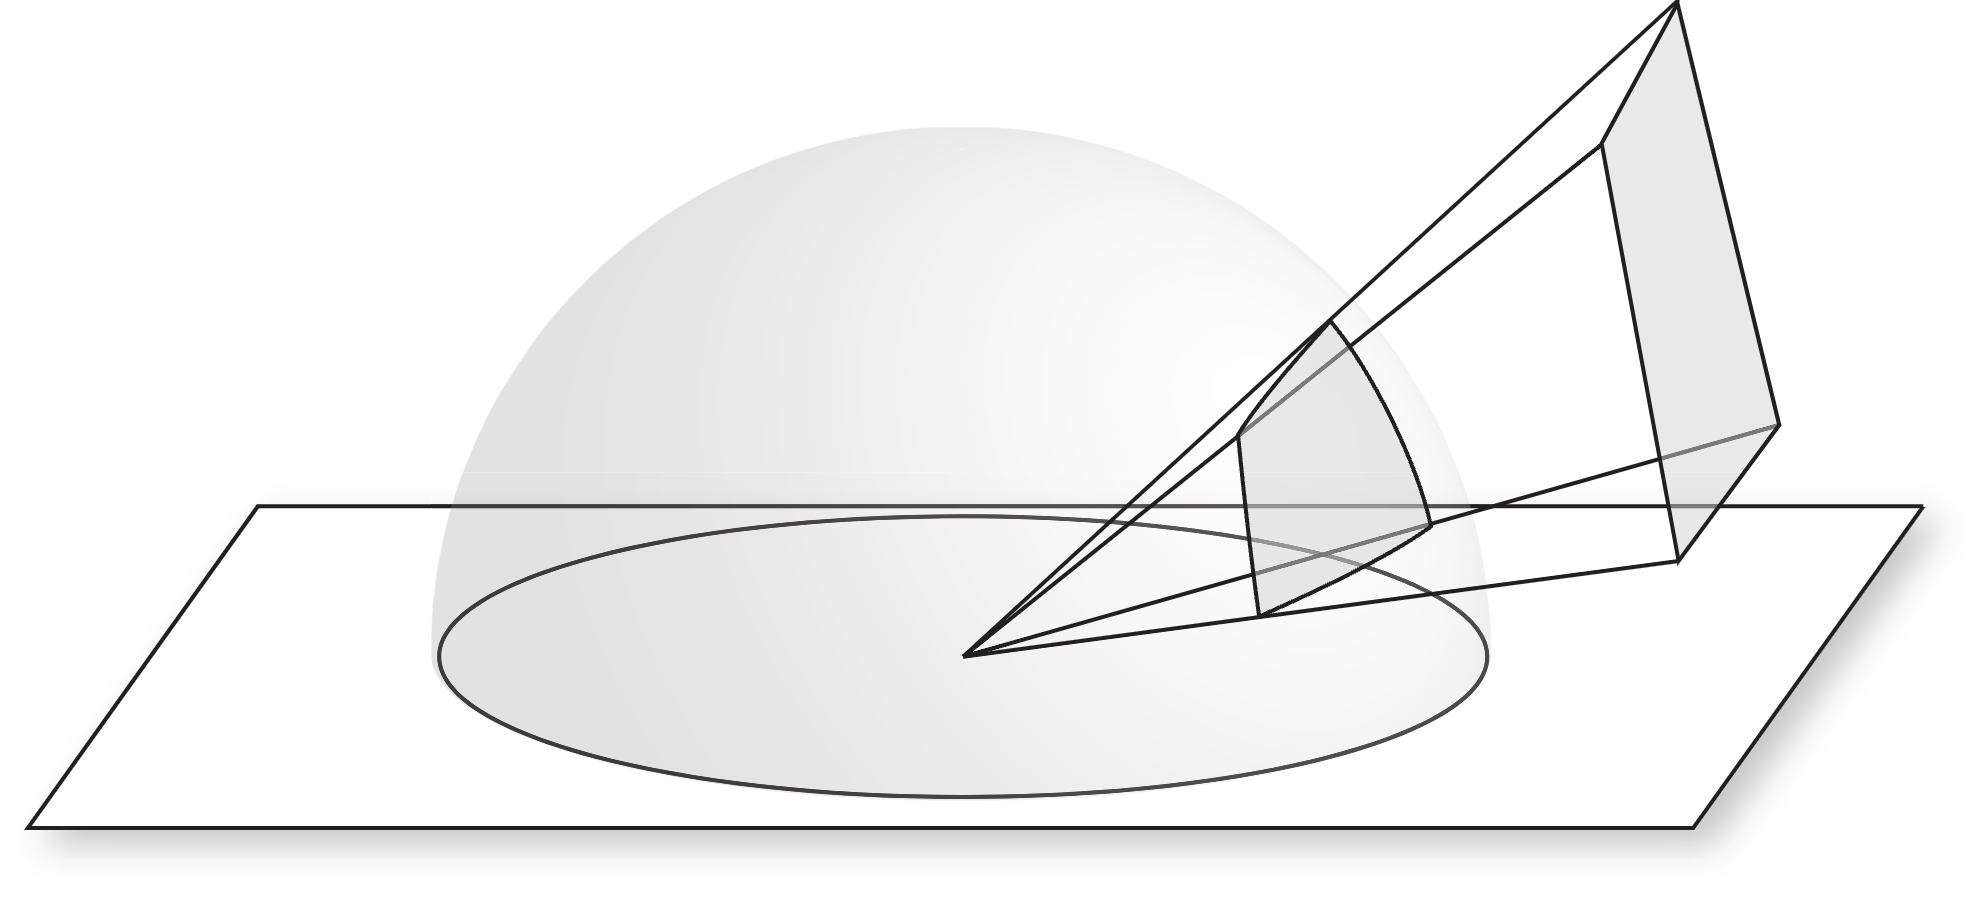
\includegraphics[width=0.7\textwidth]{images/quad_projection.png}
    \caption{Projection of quad light onto unit hemisphere from  \cite{quadonsphereprojection} }
    \label{fig:quadprojection}
\end{figure}

As illustrated in Figure \ref{fig:quadprojection}, the light source projects onto a portion of the unit hemisphere centered at our surface point (e.g. the top of one of the boxes). Our goal is to derive a PDF that correctly represents the probability of sampling any direction within this projected area.

First, consider a subsection area $dA$ on the light source. If we sample uniformly on the light, the probability of hitting this area is simply $\frac{dA}{A}$, where $A$ is the total area of the light.

Now, we need to relate this area on the light to the solid angle $d\omega$ it subtends at our surface point. The relationship between $dA$ and $d\omega$ is given by:

$$d\omega = \frac{dA \cdot \cos\theta}{r^2}$$

Where $r$ is the distance from the surface point to the sampled point on the light, and $\theta$ is the angle between the light's normal and the direction to the surface point.

The probability of sampling a direction within $d\omega$ should be equal to the probability of sampling the corresponding area $dA$ on the light. We can express this as:

$$p(\omega) \cdot d\omega = \frac{dA}{A}$$

Substituting our expression for $d\omega$:

$$p(\omega) \cdot \frac{dA \cdot \cos\theta}{r^2} = \frac{dA}{A}$$

Solving for $p(\omega)$:

$$p(\omega) = \frac{r^2}{|\cos\theta| \cdot A}$$


This derivation gives us our final PDF for sampling the light source:

$$p(\omega) = \frac{r^2}{|\cos\theta| \cdot A}$$

It accounts for the distance to the light, making distant parts less likely to be sampled, which aligns with the fact that a given solid angle corresponds to a larger area on a distant surface. It also considers the light's orientation, reducing the probability of sampling grazing angles, which project to smaller solid angles from the surface's perspective. Finally, it normalizes by the light's total area, ensuring larger lights have proportionally larger sampling probabilities.

\paragraph{Applying the PDF in Our Path Tracer}

Now that we have derived our PDF, we can correct the bias introduced by our light-sampling strategy. When we generate a sample direction towards the light, we compute the PDF value for that direction using the formula above. We then use this PDF value to divide the contribution of the sample.

By dividing by the PDF, we are effectively "turning down" the contribution of samples that were more likely to be generated (those towards the light) and "turning up" the contribution of samples that were less likely to have occurred. This correction ensures that our estimator remains unbiased despite our biased sampling strategy:

\begin{figure}[H]
    \centering
    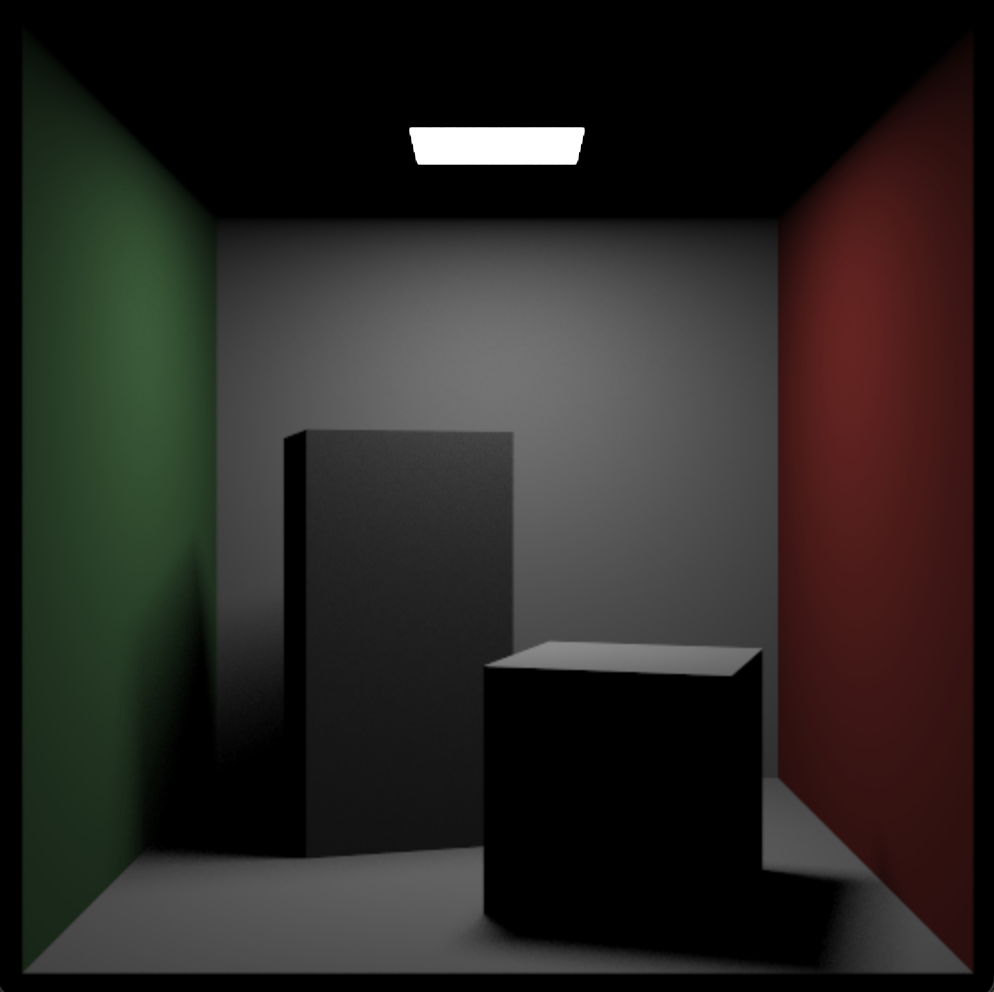
\includegraphics[width=0.5\textwidth]{images/importance_sampled.png}
    \caption{Importance Sampled Cornell Box (300 samples)}
    \label{fig:importancesampled}
\end{figure}
As illustrated in Figure \ref{fig:importancesampled}, with our PDF working in conjunction with importance sampling, we have exhibited a much better distribution of light contributions, reducing noise and enhancing the image quality with FAR fewer samples.

\subsubsection{Combining PDFs}

So great, we have a method of getting a picture of our scene very quickly. Unfortunately, in this process, we have also lost our beautiful scattered bouncing, which closely approximates realistic lighting interactions.

The easiest way to get this back is to convert our previous surface scattering into a PDF. We do this because of the awesome feature of PDFs: you can use linear mixtures to form mixture densities, which are also PDFs! Provided the probability weights all add up to one. If we combined the light sampling PDF with our hemispherical scattering PDF, we would get the best of both worlds: a very quick image converging into a very pretty image over time.


\paragraph{Lambertian Reflection as a PDF}

For Lambertian surfaces, we use a cosine-weighted Probability Density Function (PDF) to represent the scattering distribution. This aligns with Lambert's cosine law, which states that the amount of light reflected in a particular direction is proportional to the cosine angle between that direction and the surface normal.

The PDF for a Lambertian surface is given by:

$$p_{cosine}(\omega) = \frac{\max(0, \cos\theta)}{\pi}$$

Where:
$\omega$ is the direction of scattered light
$\theta$ is the angle between $\omega$ and the surface normal
$\pi$ is used for normalization

This PDF fulfils all the necessary requirements. It is normalized over the hemisphere, integrating to 1 over all possible directions. It gives a higher probability to directions closer to the surface normal, which aligns with the behaviour of diffuse surfaces and is rotationally symmetric around the surface normal. This should align with the previous explanation of shading models \ref{color_shading}.

To implement multiple importance sampling, we can combine this cosine PDF with our previously derived light sampling PDF. A simple approach is to use a weighted sum:

$$p_{combined}(\omega) = w_{light} \cdot p_{light}(\omega) + w_{cosine} \cdot p_{cosine}(\omega)$$

Where $w_{light}$ and $w_{cosine}$ are weights that sum to 1. For simplicity I will choose $w_{light} = w_{cosine} = 0.5$ to give equal importance to both strategies. Let's see how we can use this mixture PDF in our path tracer requirements:

\begin{enumerate}
    \item A method of generating a biased random direction, in our case we will flip a coin to decide which method we use here.
    \item A method that, when given a biased random direction, tells us how likely it was to be generated. A little hareder to grasp here, but as a direction could have been generated by $p_{light}(\omega)$ or $p_{cosine}(\omega)$ we take the values of BOTH PDFs, and then take the average of the weights.
\end{enumerate}


The combined PDF allows us to sample rays in a way that balances direct light sampling with the more general Lambertian scattering, resulting in this image:

\begin{figure}[H]
    \centering
    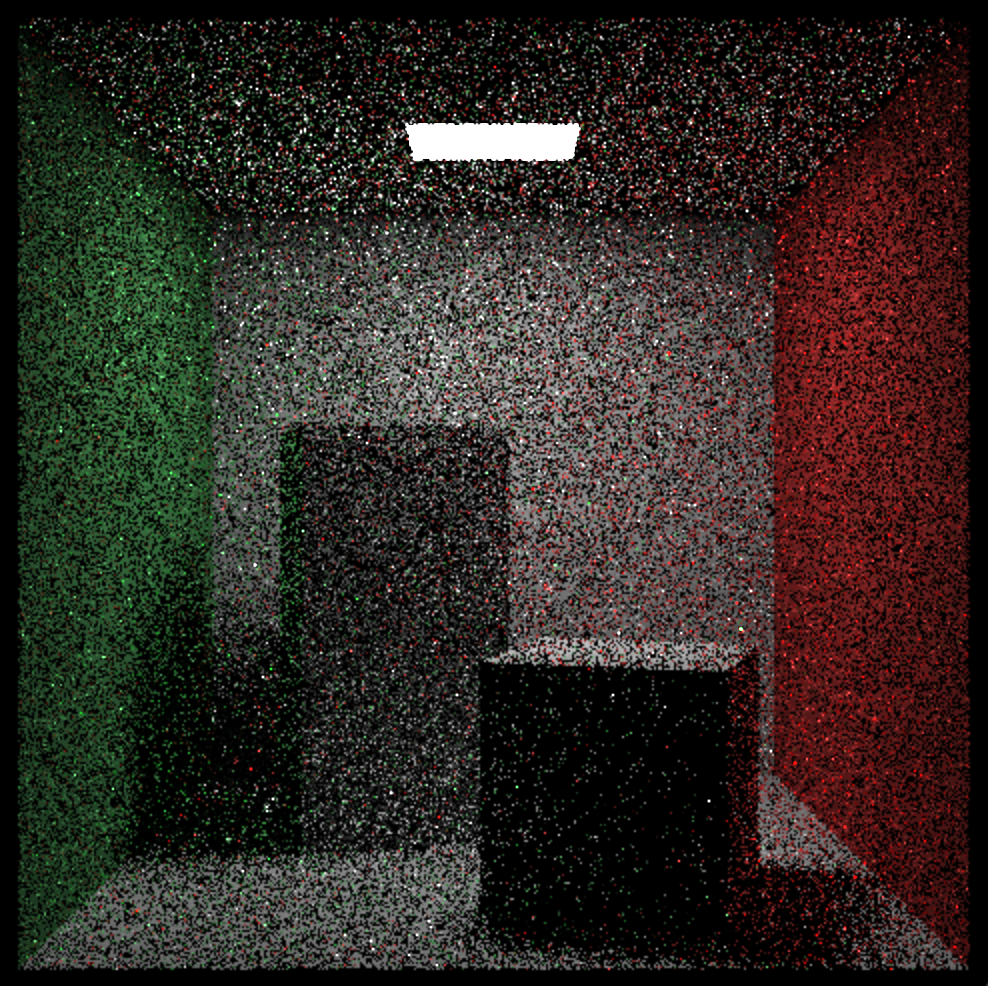
\includegraphics[width=0.5\textwidth]{images/one_samp/combined_pdf.png}
    \caption{Combined PDF Importance Sampled Cornell Box}
    \label{fig:combinedPDFimportancesampled}
\end{figure}

As you can see we have now arrived back at an image close to our original before looking into importance samwpling.

\subsection{Analysis of Results}

This does raise the point of why we bothered to go through all the maths to arrive at a very similar looking image. I will take this section to quantitatively demonstrate how much of a speed advantage we have just gained.

\paragraph{PSNR} The first metric I will use to do this is the Peak Signal-to-Noise Ratio (PSNR) which is a standard metric for assessing image quality differences \cite{imagequality}. PSNR is most easily defined via the mean squared error (MSE). Given a noise-free m×n monochrome image I and its noisy approximation K, MSE is defined as:
\[
    {\displaystyle {\mathit {MSE}}={\frac {1}{m\,n}}\sum _{i=0}^{m-1}\sum _{j=0}^{n-1}[I(i,j)-K(i,j)]^{2}.}
\]
The PSNR (in dB) is defined as:
\[
    \begin{array}{c} {\displaystyle {\begin{aligned}{\mathit {PSNR}}&=10\cdot \log _{10}\left({\frac {{\mathit {MAX}}_{I}^{2}}{\mathit {MSE}}}\right).\end{aligned}}} \end{array}
\]
Here, $MAX_I$ is the maximum possible pixel value of the image. When the pixels are represented using 8 bits per sample, this is 255. The advantage of using PSNR over MSE is that it is typically more aligned with human perception, as small differences in high dynamic range signals will have a lesser impact on the result. In comparison MSE treats all errors equally, without accounting for perceptual differences.

Shown below you can observe the visual difference between the two sampling techniques we covered, with the final image showcasing the pixels that have changed color (in red).

\begin{figure}[H]
    \centering
    \begin{subfigure}[t]{0.32\textwidth}
        \centering
        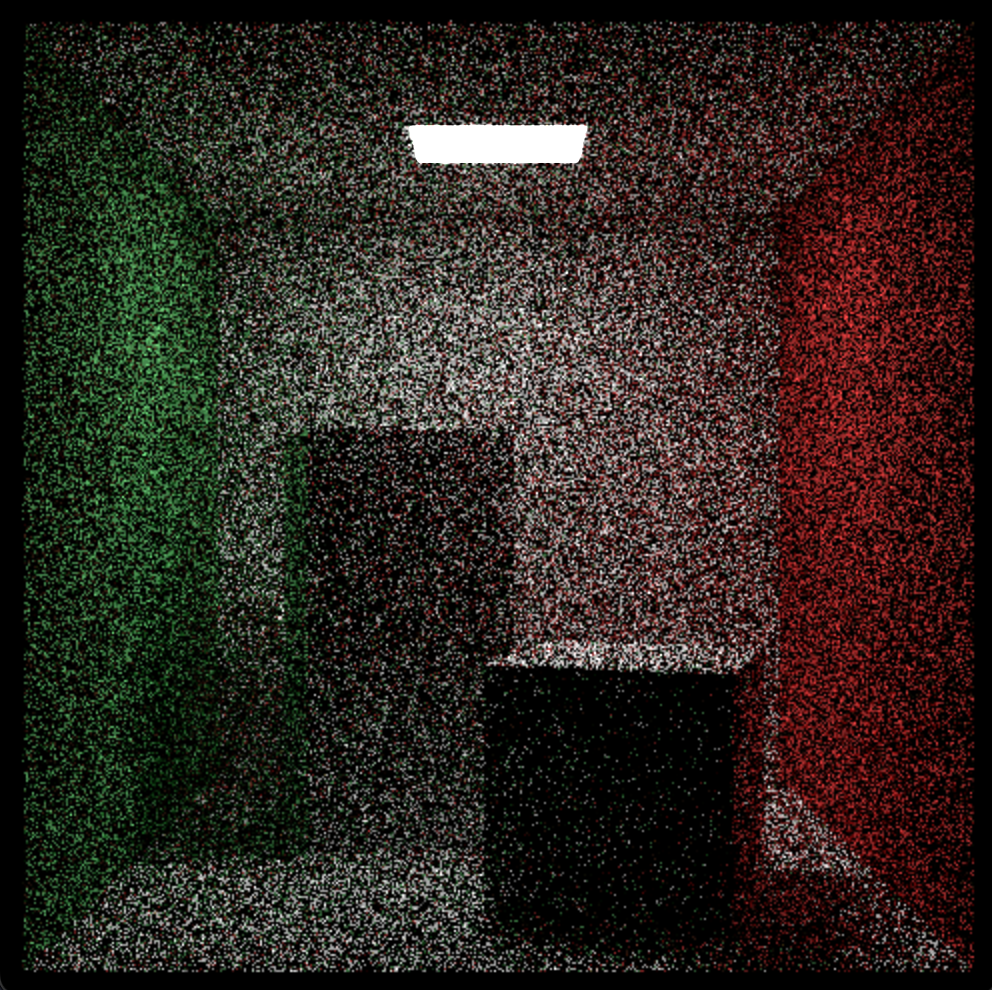
\includegraphics[width=\textwidth]{images/25_samp/randomPDF.png}
        \caption{Naive path tracing}
        \label{fig:naive_sampling}
    \end{subfigure}
    \hfill
    \begin{subfigure}[t]{0.32\textwidth}
        \centering
        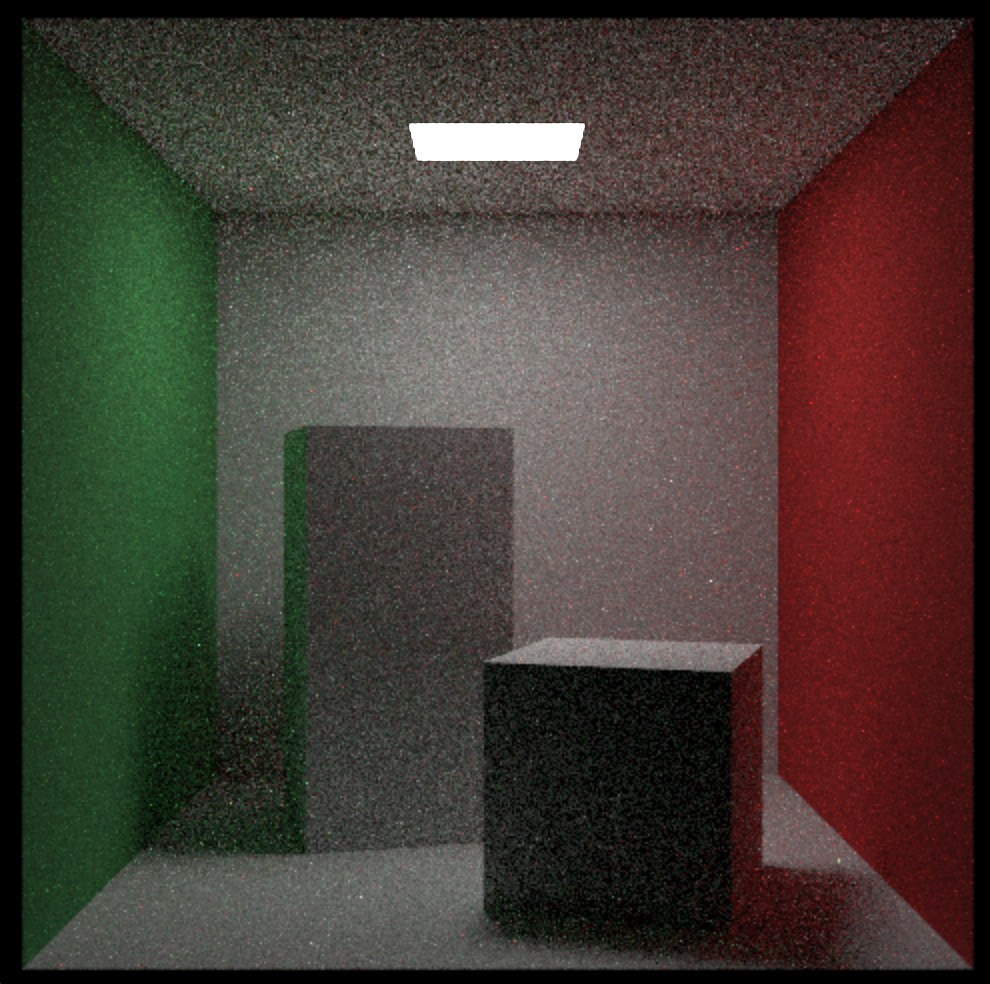
\includegraphics[width=\textwidth]{images/25_samp/combPDF.png}
        \caption{Multiple Importance Sampling}
        \label{fig:mis_sampling}
    \end{subfigure}
    \hfill
    \begin{subfigure}[t]{0.32\textwidth}
        \centering
        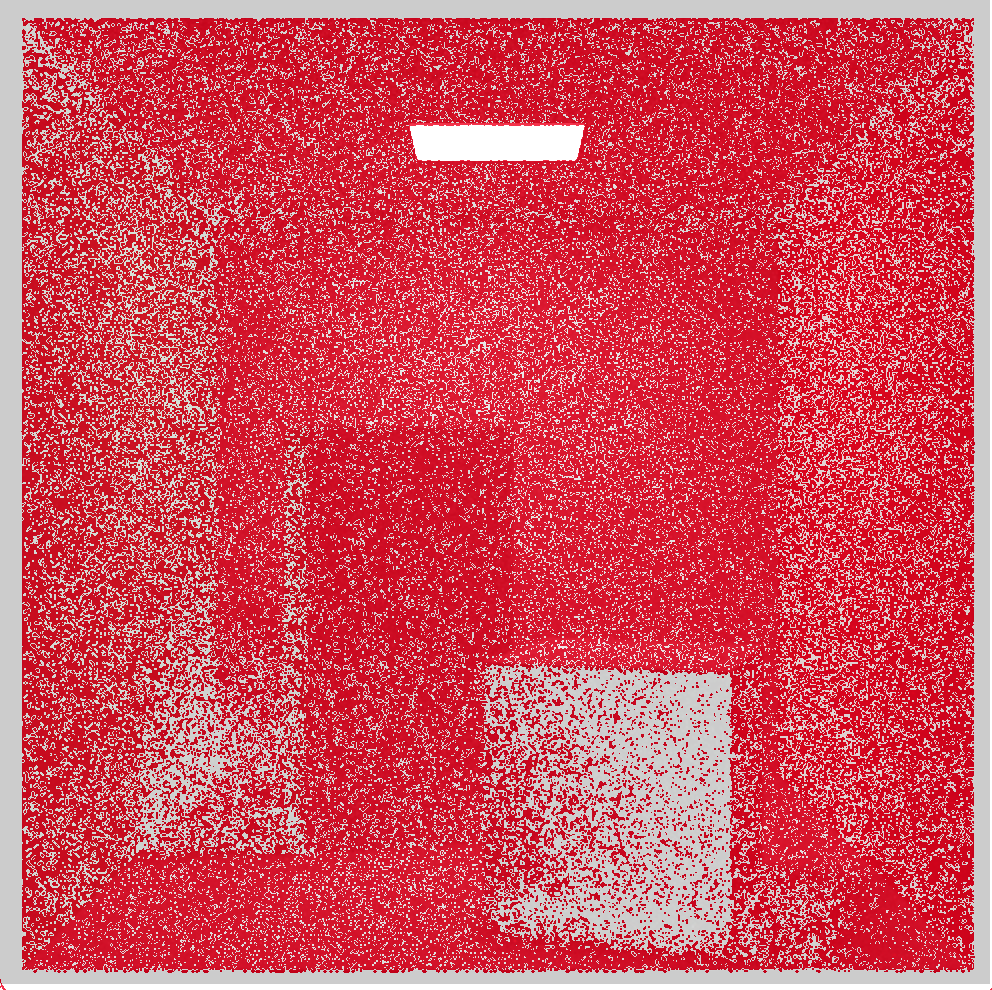
\includegraphics[width=\textwidth]{images/25_samp/comparison.png}
        \caption{Pixels changed (fuzz of 10\%)}
        \label{fig:comparison}
    \end{subfigure}
    \caption{Comparison of naive path tracing vs.\ Multiple Importance Sampling (Both 25 samples per pixel)}
    \label{fig:sampling_comparison}
\end{figure}

In Figure \ref{fig:sampling_comparison}, we can observe that the MIS approach (Figure \ref{fig:mis_sampling}) produces a cleaner image with less noise, particularly in areas of indirect illumination and near light sources. The naive approach (Figure \ref{fig:naive_sampling}) struggles with high-variance estimates in these regions, resulting in a noisier image.

If we take the PSNR value between the two of these image we get 16.9 dB. PSNR values for image comparisons typically range from 20 to 40 dB, with a PSNR of 30-40 dB being considered acceptable for high-quality images. This means our value of 16.9 dB reflects a \textit{substantial} discrepancy between the MIS approach and the naive approach.


\paragraph{Render time} Next I will look at the time required to render each frame (an obviously crucial metric). The times recorded were as follows:
\begin{enumerate}
    \item Random Scattering Sampling:
          156.8 seconds to render the image with an average frame render time of 6.27 seconds.

    \item Combined PDF Importance Sampling:
          78.7 seconds to render the image with an average frame render time of 3.14 seconds.
\end{enumerate}

Thus we can conclude that by implementing importance sampling we have decreased the speed to render a frame of our image by approximately 50\%!.

These two metrics demonstrate that the Combined PDF Importance Sampling method is not only significantly quicker but also offers huge improvements in image quality.
It should be stressed here that \textit{both methods ultimately produce the same final image}, it is just that our importance sampling achieves this outcome MUCH faster.

\pagebreak
\section{Technical Description of the System}
\label{sec:system-description}

I have now finished in my imparting of path-tracer specific knowledge, and will change to a description of how one might build and architect the topics covered in this paper. It would be helpful if the reader would have knowledge of C++ and OpenGL, as I will include some code snippets.

\subsection{System Architecture}

\paragraph{Design Principles Behind the Modular Architecture} Before architecting a complex system, keeping several non-functional attributes in mind and continually assessing your architectural decisions against these is essential.
A path tracer requires several key non-functional attributes (ordered by descending importance):

\begin{enumerate}
    \item Performance: The system must handle complex scenes and produce high-quality renders in a reasonable time frame.
    \item Extensibility: As rendering techniques evolve, the system should be able to incorporate new algorithms and features quickly.
    \item Maintainability: The codebase should be easy to understand, debug, and modify.
\end{enumerate}

These requirements naturally lead to a modular monolith approach. I find that modular design is suited to our non-functional attributes as it allows for the developer to have clear interfaces between modules, making it easier to modify or replace individual components without affecting the entire system (imagine you want to switch to the Vulkan API, this should be quite an easy task!). This approach is particularly well-suited for a path tracer, where tight integration between components is necessary for performance. However, a clear separation of concerns is crucial for ongoing development and maintenance.

\paragraph{Overview of Core Components and Their Interactions}

The following C4 diagram provides an overview of the path tracer's modules, along with their responsibilities and interactions:

\begin{figure}[H]
    \centering
    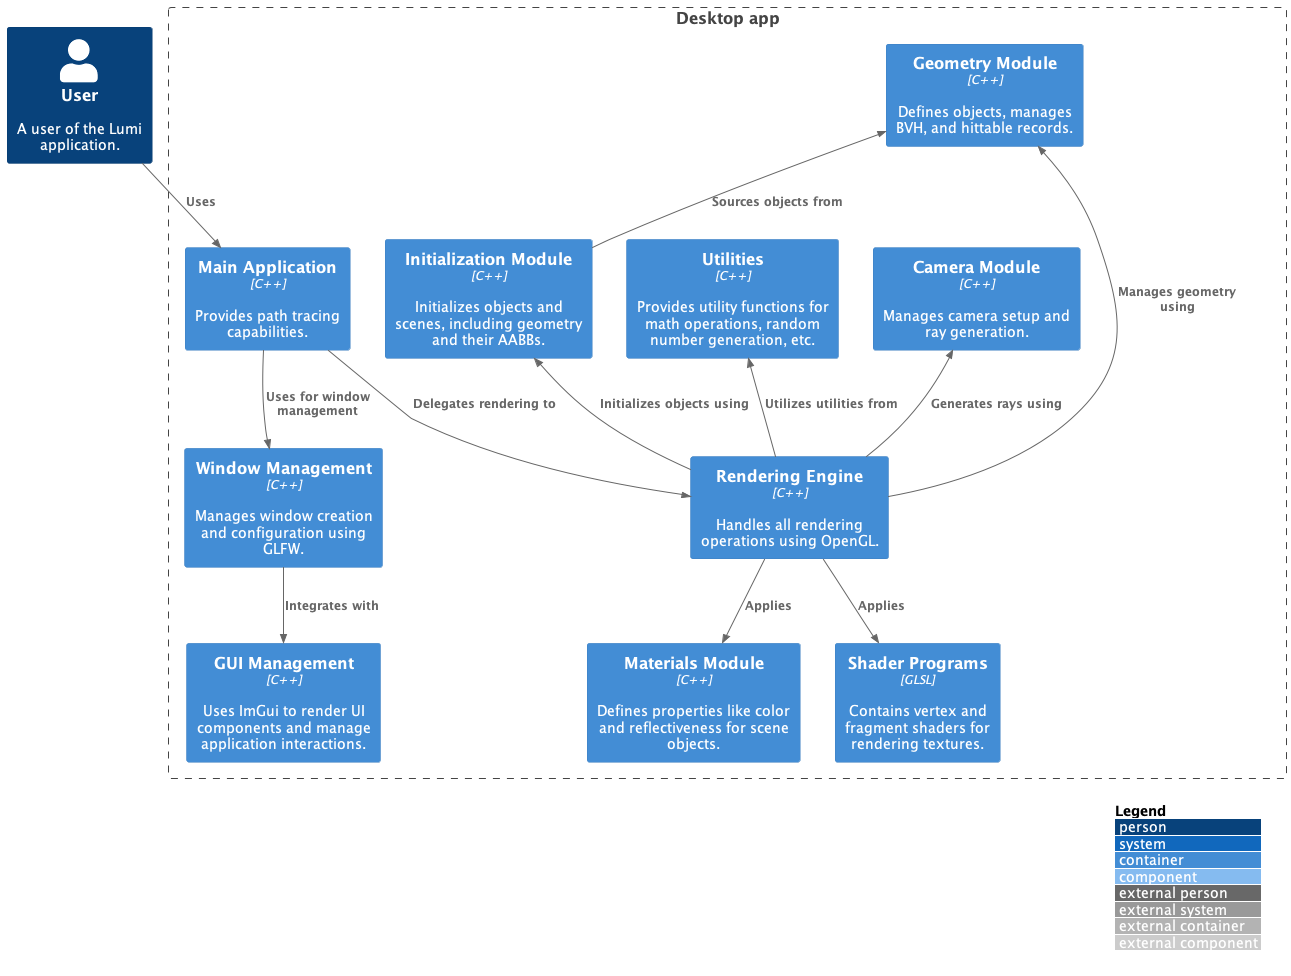
\includegraphics[width=\textwidth]{images/software_architecture/lumi_pml.png}
    \caption{C4 diagram of the path tracer system architecture}
    \label{fig:c4-diagram}
\end{figure}

The main loop initialises the GLFW window we use for displaying the image, and summons the renderer to start.
The Rendering Engine acts as the central hub, coordinating the activities of other modules. Below we can trace the renderer's dependencies in the path tracing code:

\begin{figure}[H]
    \centering
    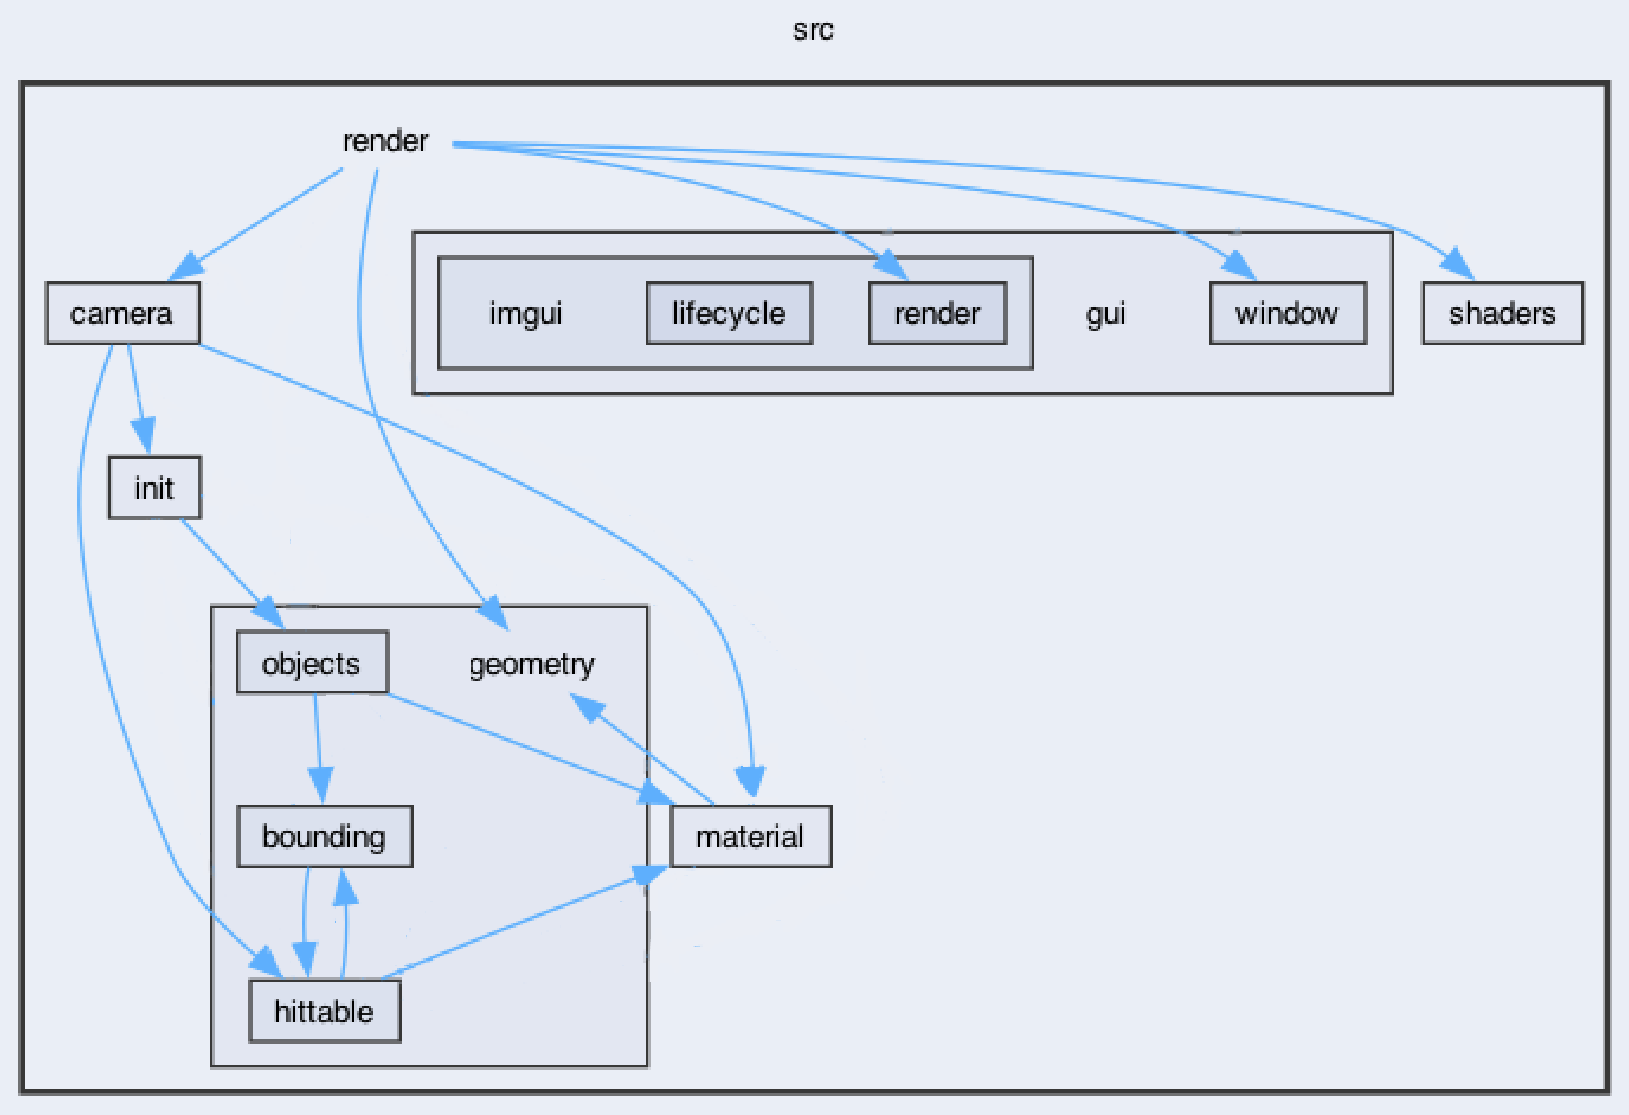
\includegraphics[width=\textwidth]{images/software_architecture/directory_dependencies.png}
    \caption{Renderer's dependencies in code}
    \label{fig:rendererdependency}
\end{figure}


Here, we notice all the other modules in use, with the camera module providing its properties via its init method and generating the primary rays. These rays, in turn, will depend on the Geometry folder, which provides the Abstraction for Hittable Objects and the interface to interact with these.

We can also notice a neat division of modularity here; all code related to window management, including any GUI, is entirely encapsulated, and \textbf{only} depended on by our renderer. This makes switching technologies extremely easy if needed.

\paragraph{Procedure calls}  The runtime of the path tracer can be best understood by examining the main renderer's call stack and the specific process of ray-object intersection.
\begin{figure}[H]
    \centering
    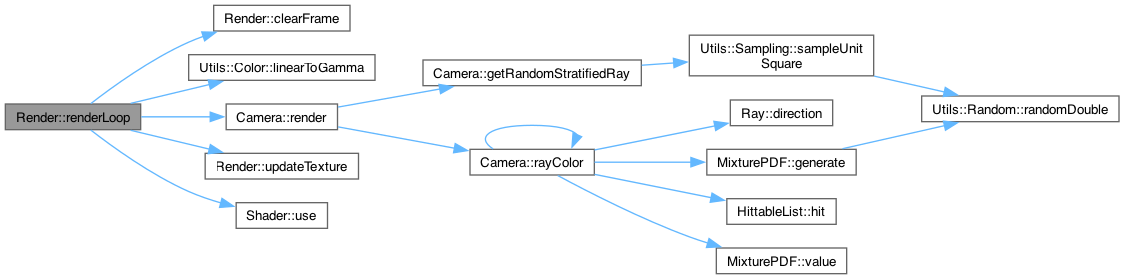
\includegraphics[width=\textwidth]{images/software_architecture/render_loop_call.png}
    \caption{Diagram of the renderer's call stack}
    \label{fig:renderercallstack}
\end{figure}

\begin{enumerate}
    \item \textbf{Render::renderLoop} initiates the process. Within the loop:
          \begin{description}
              \item[Render::clearFrame] Clears the window
              \item[Utils::Color::linearToGamma] Color accuracy conversion
              \item[Camera::render] Generates the image
              \item[Shader::use] Applies the shaders to the window
              \item[Render::updateTexture] Updates the window
          \end{description}

    \item \textbf{Camera::render} generates rays using \textbf{Camera::getRandomStratifiedRay} for stratified sampling.

    \item For each ray:
          \begin{description}
              \item[Ray::direction] Computes ray path
              \item[Camera::rayColor] Calculates color contribution
              \item[MixturePDF] Implements importance sampling (both generating a ray and getting its PDF Value)
              \item[HittableList::hit] Tests for object intersections
          \end{description}

    \item Recursive calls to \textbf{Camera::rayColor} handle light bounces.
\end{enumerate}
This structure incorporates stratified sampling, importance sampling, and recursive ray tracing for global illumination.

Here we find an example of a ray intersecting with an object (specifically a quad):

\begin{figure}[H]
    \centering
    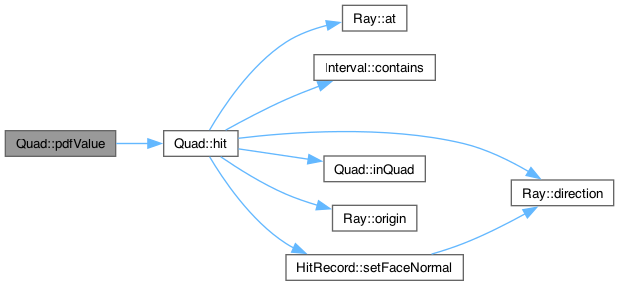
\includegraphics[width=\textwidth]{images/software_architecture/quad_loop_call.png}
    \caption{Diagram of a quad's call stack}
    \label{fig:quadcallstack}
\end{figure}

\begin{enumerate}
    \item \textbf{Quad::hit} initiates the intersection test.

    \item Ray properties used:
          \begin{description}
              \item[Ray::at] determines the ray's position.
              \item[Ray::origin] and \textbf{Ray::direction} establish the ray's start and trajectory.
          \end{description}

    \item Intersection checks:
          \begin{description}
              \item[Interval::contains] verifies the intersection is within a valid range.
              \item[Quad::inQuad] confirms the intersection is within the quad's boundaries.
          \end{description}

    \item \textbf{HitRecord::setFaceNormal} sets the intersected face normal for shading calculations.
\end{enumerate}

Notice how this architecture, with applied SOLID principles, allows us to provide a robust foundation and remain adaptable to future enhancements. An example would be implementing a Bounding Volume Hierarchy for more efficient ray intersections. This could very quickly be "slotted" into our existing architecture (which I have done in the program's source code)

\subsection{Utilising OpenGL for Visualising Convergence}


The final subject I wish to tackle in this paper is a "debug mode" I have added to the path tracer, which was very helpful during its development. The entire path tracer runs on the CPU currently (much slower than a GPU, but \textit{far} easier to develop), and thus, we have no easy method of quickly rendering to a screen (versus simply writing to an image file). We currently cannot provide any insight into the image's gradual convergence process. To address this limitation, I implemented a progressive rendering system using OpenGL (utilising the GPU), allowing for real-time visualisation of the path tracing process.

\paragraph{Progressive Rendering} The core of this visualization technique is an accumulation buffer. Instead of directly outputting the final pixel colors after x amounts of samples per pixel, I continuously update an accumulation buffer:

\begin{minted}{cpp}
vector<vec3> accumulationBuffer(IMAGE_SIZE, 0);
vector<int> sampleCount(IMAGE_SIZE, 0);
\end{minted}

This \texttt{accumulationBuffer} stores the sum of all samples for each pixel, while the \texttt{sampleCount} keeps track of the number of samples per pixel. This allows us to at any point calculate the state of the current images pixels:
\begin{minted}{cpp}
currentImage[i] = accumulationBuffer[i] / sampleCount[i];
\end{minted}

We update the accumulation buffer after each sample via this code:

\begin{minted}{cpp}
accumulationBuffer[index] += rayColor(r, world, maxDepth);
sampleCount[index] += 1;
\end{minted}

To display the progressively rendered image, we utilize OpenGL's texture mapping capabilities.
The current state of the rendered image is mapped to a texture that covers the entire window:

\begin{minted}{cpp}
void updateTexture(unsigned int texture, const vector<vec3> &image,
    const int &WIDTH, const int &HEIGHT)
    {
        glBindTexture(GL_TEXTURE_2D, texture);
        glTexSubImage2D(WIDTH, HEIGHT, image.data());
    }
\end{minted}

From there we map to a uniform in our fragment shader:

\begin{minted}{cpp}
uniform sampler2D screenTexture;
void main()
{
    FragColor = texture(screenTexture, TexCoord);
}
\end{minted}

The advantage here is that a simple CPU-path-traced application can utilise the GPU as an intermediate representation. Thus, we can skip the extensive effort of converting our Cpp code to shader code. This has made the Path tracer's development process significantly easier, making it easier to identify and debug issues in the path tracing algorithm. One area of consideration is the amount of time to transfer the data from the CPU to the GPU; if we were to do this 100 times a second, this would be very slow and laggy. I found that updating the window once per full viewport render was good enough.

\section{Conclusion}
\label{sec:conclusion}
\subsection{Summary of Key Points}
In this report, I tried to lay out the foundations of everything a path tracer is and ended up using Monte Carlo methods to simulate realistic lighting in a 3D scene. I hope I have illustrated the effectiveness of this technique, especially in the speed and quality of the rendered images, making the path tracer both computationally efficient and visually realistic.

\subsection{Future Work}

While this work has demonstrated the power of path tracing, there remain many opportunities for further enhancement and exploration, some of which include:
\begin{itemize}
    \item Bounding Volume Hierarchies (BVH): While the codebase includes an implementation, this report did not cover BVH in detail. Future work could focus on optimising BVH construction and traversal to improve performance, essential in scenes with complex geometries.

    \item Support for .obj File Handling: Incorporating functionality for reading and rendering more complex object geometries from .obj files would allow us to make much more diverse scenes (like the Stanford Bunny \cite{stanfordbunny}!).

    \item Transition to GPU Rendering: Migrating the path tracing computations to the GPU could significantly reduce rendering times and enable real-time applications.
\end{itemize}

In a more general sense, I recommend exploring graphics papers (both old and new!) and seeing if you can implement any of the techniques they talk about. In particular, I am a fan of Nvidia's and Pixar's papers. Happy reading!

\section{References}
\label{sec:references}
\bibliographystyle{plain}
\bibliography{references}

\appendix
\section{Detailed Mathematics}
\label{sec:appendix-derivations}

\subsection{Linearity of Transformations}
\label{sec:appendix-derivations-linear}
To demonstrate why translation is not a linear transformation, we consider the following properties: \\

Law of Additivity: \( T(\mathbf{u} + \mathbf{v}) = T(\mathbf{u}) + T(\mathbf{v}) \)

Law of Homogeneity: \( T(c\mathbf{u}) = cT(\mathbf{u}) \)

If we test the linearity conditions:

Additivity:
\[
    T(\mathbf{u} + \mathbf{v}) = (\mathbf{u} + \mathbf{v}) + \mathbf{b} \neq T(\mathbf{u}) + T(\mathbf{v}) = (\mathbf{u} + \mathbf{b}) + (\mathbf{v} + \mathbf{b})
\]

The right-hand side becomes \( \mathbf{u} + \mathbf{v} + 2\mathbf{b} \), which is not equal to the left-hand side.

Homogeneity:
\[
    T(c\mathbf{u}) = c\mathbf{u} + \mathbf{b} \neq cT(\mathbf{u}) = c(\mathbf{u} + \mathbf{b}) = c\mathbf{u} + c\mathbf{b}
\]

The translation vector \( \mathbf{b} \) remains unchanged and doesn’t scale with \( c \), breaking this property as well.

Thus, the translation is an affine transformation, not a linear transformation, because it doesn’t preserve these linearity conditions.

\subsection{Derivation of Rotation Matrices}
\label{sec:appendix-derivations-rotation}

To derive rotation matrices, we start by considering rotation in a 2D plane, which forms the basis for 3D rotations. In 3D space, rotation around any axis can be decomposed into rotations in the planes perpendicular to that axis.

\subsubsection{2D Rotation}

Lets consider a point $(x, y)$ in a 2D plane. We can also represent this point in polar coordinates $(x = r \cos\phi,  y = r \sin\phi)$.

When rotated counterclockwise by an angle $\theta$ around the origin, its new coordinates $(x', y')$ can be expressed as:
$$
    \begin{aligned}
        x' = r \cos(\phi + \theta) \\
        y' = r \sin(\phi + \theta)
    \end{aligned}
$$
We can then use the trigonemtric sum and difference identities to expand:

$$
    \begin{aligned}
        x' & = r \cos(\phi + \theta) = r \cos\phi \cos\theta - r \sin\phi \sin\theta = x \cos\theta - y \sin\theta \\
        y' & = r \sin(\phi + \theta) = r \sin\phi \cos\theta + r \cos\phi \sin\theta = x \sin\theta + y \cos\theta
    \end{aligned}
$$

This 2D rotation can now be represented as a matrix:

$$
    \begin{pmatrix}
        x' \\ y'
    \end{pmatrix} =
    \begin{bmatrix}
        \cos\theta & -\sin\theta \\
        \sin\theta & \cos\theta
    \end{bmatrix}
    \begin{pmatrix}
        x \\ y
    \end{pmatrix}
$$

\subsubsection{3D Rotations}

Now, we'll extend this concept to 3D rotations around each axis.

\paragraph{X-Axis} When rotating around the x-axis:
\begin{itemize}
    \item The x-coordinate remains unchanged.
    \item The y and z coordinates rotate in the yz-plane.
\end{itemize}

Applying the 2D rotation to the yz-plane:

$$
    \begin{aligned}
        x' & = x                           \\
        y' & = y \cos\theta - z \sin\theta \\
        z' & = y \sin\theta + z \cos\theta
    \end{aligned}
$$

This yields the matrix $\mathbf{R}_x(\theta)$:

$$
    \mathbf{R}_x(\theta) = \begin{bmatrix}
        1 & 0          & 0           & 0 \\
        0 & \cos\theta & -\sin\theta & 0 \\
        0 & \sin\theta & \cos\theta  & 0 \\
        0 & 0          & 0           & 1
    \end{bmatrix}
$$


\paragraph{Y-Axis} For rotation around the y-axis:
\begin{itemize}
    \item The y-coordinate remains unchanged.
    \item The x and z coordinates rotate in the xz-plane.
\end{itemize}

However, we must be careful here. The positive rotation around the y-axis is defined as counterclockwise when looking down the y-axis from positive to negative. This means in the xz-plane, positive rotation appears clockwise. Therefore, we need to negate the angle in our 2D rotation formula:

$$
    \begin{aligned}
        x' & = x \cos(-\theta) - z \sin(-\theta) = x \cos\theta + z \sin\theta  \\
        y' & = y                                                                \\
        z' & = x \sin(-\theta) + z \cos(-\theta) = -x \sin\theta + z \cos\theta
    \end{aligned}
$$

This gives us the matrix $\mathbf{R}_y(\theta)$:

$$
    \mathbf{R}_y(\theta) = \begin{bmatrix}
        \cos\theta  & 0 & \sin\theta & 0 \\
        0           & 1 & 0          & 0 \\
        -\sin\theta & 0 & \cos\theta & 0 \\
        0           & 0 & 0          & 1
    \end{bmatrix}
$$

\paragraph{Z-Axis} For rotation around the z-axis:
\begin{itemize}
    \item The z-coordinate remains unchanged.
    \item The x and y coordinates rotate in the xy-plane.
\end{itemize}

This directly applies our 2D rotation:

$$
    \begin{aligned}
        x' & = x \cos\theta - y \sin\theta \\
        y' & = x \sin\theta + y \cos\theta \\
        z' & = z
    \end{aligned}
$$

Resulting in the matrix $\mathbf{R}_z(\theta)$:

$$
    \mathbf{R}_z(\theta) = \begin{bmatrix}
        \cos\theta & -\sin\theta & 0 & 0 \\
        \sin\theta & \cos\theta  & 0 & 0 \\
        0          & 0           & 1 & 0 \\
        0          & 0           & 0 & 1
    \end{bmatrix}
$$

After going through the 3D rotation matrices step-by-step I find it a lot less scary, at the very least it's quite clear how they emerge from 2D.
We then of course make the fourth row and column in each matrix all zeros (except for a 1 in the diagonal), which allow these rotations to be combined with other transformations in homogeneous coordinates.

\end{document}
